%=============================================================================
\documentclass[10pt,a4paper]{article}
%
%
%
%
\usepackage{graphicx}
\usepackage{hyperref}
\usepackage{verbatim}
\usepackage{fix-cm}
\usepackage{lineno}
\usepackage{fancyhdr}
%\usepackage{amsmath}
%
\oddsidemargin  0.1 in
\evensidemargin 0.1 in
%
%
\newlength{\backindent}\setlength{\backindent}{2cm}
\textwidth 5.375 in % Width of text line.
\advance\textheight by1.4cm
\advance\voffset by-1.4cm
\advance\textwidth by\backindent
%
%
% === Fancy headers setup  ===============================
%
\setlength{\headheight}{15.2pt}
\pagestyle{fancyplain} {
\fancyhead[L]{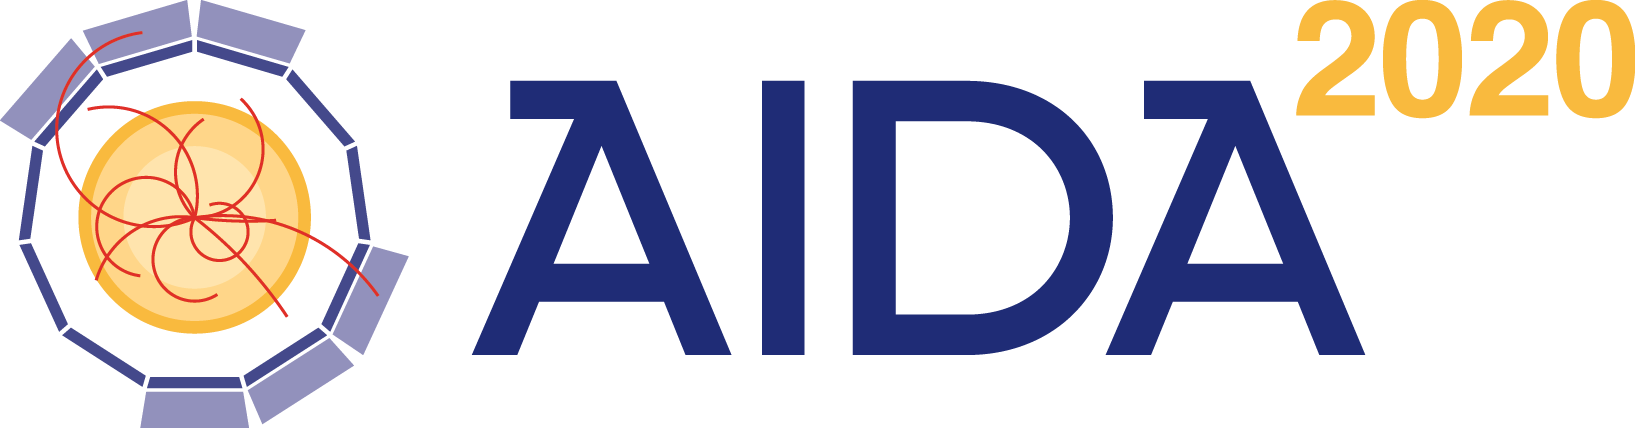
\includegraphics[height=10mm]{./setup/AIDA2020-logo}\vspace{-0.3cm}}
\fancyhead[C]{}
\fancyhead[R]{\sffamily{\underline{\hspace{6cm}Advanced European Infrastructures for Detectors at Accelerators}}}
\fancyfoot[L]{}
\fancyfoot[C]{\sffamily{User Manual}}
\fancyfoot[R]{\sffamily{\thepage}}
}
%
%
\newcommand{\tw}[1]{${\tt{#1}}$}
\newcommand{\tts}[1]{{\tt\small{#1}}}
\newcommand{\bold}[1]{{\bf{#1}}}
%
%
\newcommand{\docline}[2]{\vspace{0.1cm}{\bf{#1}} & \parbox{14.5cm}{#2}\\}
%
% === Specialization of the lineno package
%
\renewcommand{\linenumberfont} {\normalfont\small\sffamily}
\renewcommand{\makeLineNumber} {\makeLineNumberLeft}
\renewcommand{\linenumbersep} {2pt}
%
% === Set font to code section with line numbers
%
\newenvironment{code}{\par\vspace{0.01cm}\small\linenumbers\verbatim\setcounter{linenumber}{1}}{\endverbatim\nolinenumbers\vspace{-0.02cm}}%
%
% === Set font to code section with line numbers
%
\newenvironment{unnumberedcode}{\par\vspace{-0.1cm}\small\verbatim\setcounter{linenumber}{1}}%
{\endverbatim\vspace{-0.2cm}}
%
%
% ===  Compactify the item list  =========================
%
\newcommand{\itemcompact}{\setlength{\itemsep}{1pt}\setlength{\parskip}{0pt}\setlength{\parsep}{0pt}}
%
%
% ===  Title page command  ===============================
%
%
\newcommand{\basictitle}[2]{
%
\pagestyle{empty}
%
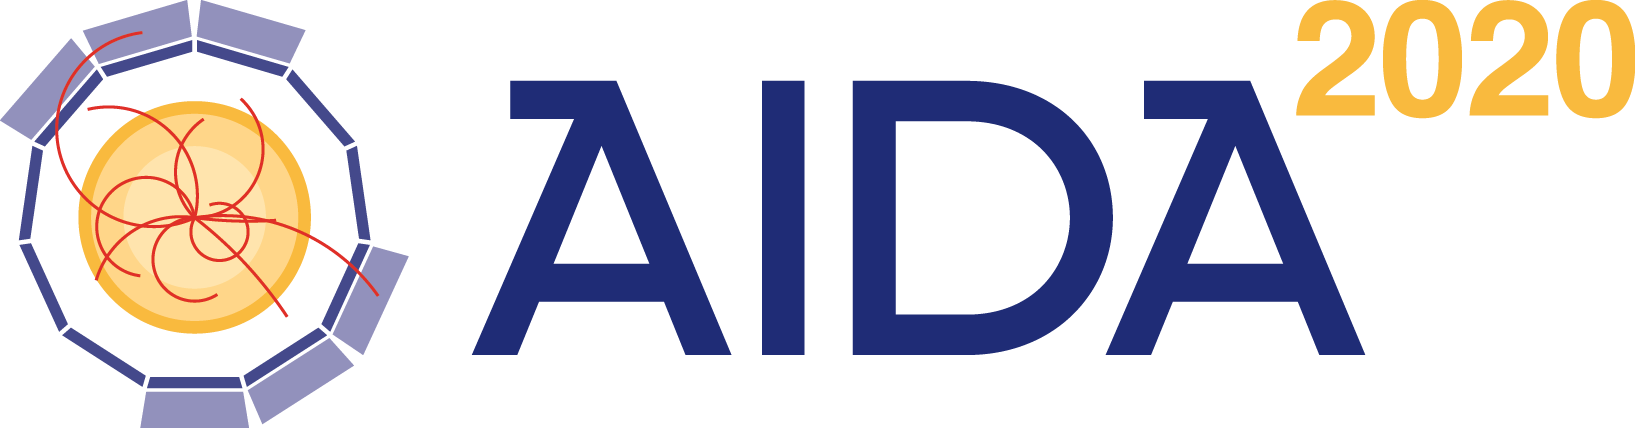
\includegraphics[height=25mm] {./setup/AIDA2020-logo}

\vspace{0.02cm}

{\sffamily{\underline{\hspace{6cm}Advanced European Infrastructures for Detectors at Accelerators}}}

\vspace{2cm}

\begin{center}
{\fontsize{72}{32}\selectfont{\bfseries{#1}}}

\vspace{3cm}
{\Huge\bf{#2}}
\vspace{3cm}
\begin{figure}[b]
  \begin{center}
    
\includegraphics[height=15mm] {./setup/Horizon2020-grant-logo}
  \end{center}
\end{figure}
\end{center}
}
\newcommand{\AIDAtitle}[3]{
\begin{titlepage}
\basictitle{#1}{#2}
\begin{center}
{#3}
\end{center}
\end{titlepage}
}

%
% === Command to insert http links to the DD4hep geomtery package
%
\newcommand{\detdesc}[2]
{
    \href{http://www.cern.ch/frankm/DD4hep/#1}{#2}
}
%
% === Command to insert http links to the ROOT geomtery package
%
\newcommand{\tgeo}[2]
{
    \href{http://root.cern.ch/root/html/#1.html}{#2}
}
\newcommand{\tgeoO}[3]
{
    \href{http://root.cern.ch/root/html/#1:#2}{#3}
}
\newcommand{\DDE}{{$\tt{DDEve}$\space}}
\newcommand{\DDhep}{{$\tt{DD4hep}$\space}}
\newcommand{\DDH}{{$\tt{DD4hep}$\space}}
\newcommand{\DDG}{{\tt{DDG4}\space}}
\newcommand{\DDA}{{\tt{DDAlign}\space}}
\newcommand{\DDC}{{\tt{DDCond}\space}}
\newcommand{\DDR}{{\tt{DDRec}\space}}
%
% ===  Custom title page  ================================
%
\newcommand{\mytitle}[3]{
\begin{titlepage}
\basictitle{#1}{#2}
\begin{center}
{#3}
\end{center}
\end{titlepage}
}

%
%
\usepackage{graphicx}
\usepackage{hyperref}
\usepackage{verbatim}
\usepackage{fix-cm}
\usepackage{lineno}
\usepackage{fancyhdr}
%\usepackage{amsmath}
%
\oddsidemargin  0.1 in
\evensidemargin 0.1 in
%
%
\newlength{\backindent}\setlength{\backindent}{2cm}
\textwidth 5.375 in % Width of text line.
\advance\textheight by1.4cm
\advance\voffset by-1.4cm
\advance\textwidth by\backindent
%
%
% === Fancy headers setup  ===============================
%
\setlength{\headheight}{15.2pt}
\pagestyle{fancyplain} {
\fancyhead[L]{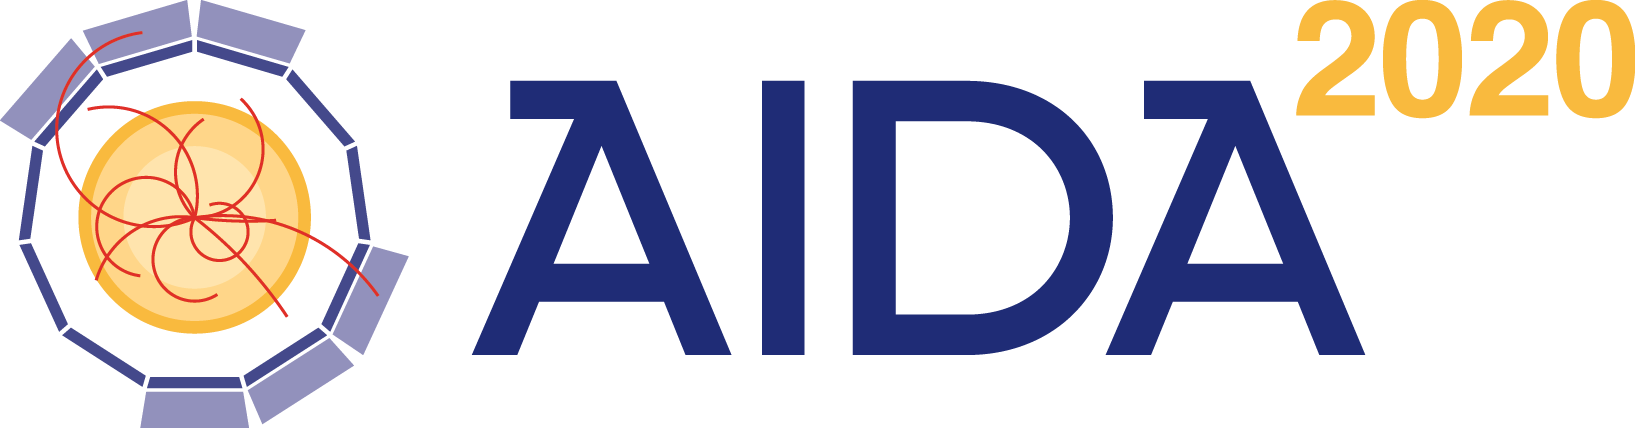
\includegraphics[height=10mm]{./setup/AIDA2020-logo}\vspace{-0.3cm}}
\fancyhead[C]{}
\fancyhead[R]{\sffamily{\underline{\hspace{6cm}Advanced European Infrastructures for Detectors at Accelerators}}}
\fancyfoot[L]{}
\fancyfoot[C]{\sffamily{User Manual}}
\fancyfoot[R]{\sffamily{\thepage}}
}
%
%
\newcommand{\tw}[1]{${\tt{#1}}$}
\newcommand{\tts}[1]{{\tt\small{#1}}}
\newcommand{\bold}[1]{{\bf{#1}}}
%
%
\newcommand{\docline}[2]{\vspace{0.1cm}{\bf{#1}} & \parbox{14.5cm}{#2}\\}
%
% === Specialization of the lineno package
%
\renewcommand{\linenumberfont} {\normalfont\small\sffamily}
\renewcommand{\makeLineNumber} {\makeLineNumberLeft}
\renewcommand{\linenumbersep} {2pt}
%
% === Set font to code section with line numbers
%
\newenvironment{code}{\par\vspace{0.01cm}\small\linenumbers\verbatim\setcounter{linenumber}{1}}{\endverbatim\nolinenumbers\vspace{-0.02cm}}%
%
% === Set font to code section with line numbers
%
\newenvironment{unnumberedcode}{\par\vspace{-0.1cm}\small\verbatim\setcounter{linenumber}{1}}%
{\endverbatim\vspace{-0.2cm}}
%
%
% ===  Compactify the item list  =========================
%
\newcommand{\itemcompact}{\setlength{\itemsep}{1pt}\setlength{\parskip}{0pt}\setlength{\parsep}{0pt}}
%
%
% ===  Title page command  ===============================
%
%
\newcommand{\basictitle}[2]{
%
\pagestyle{empty}
%
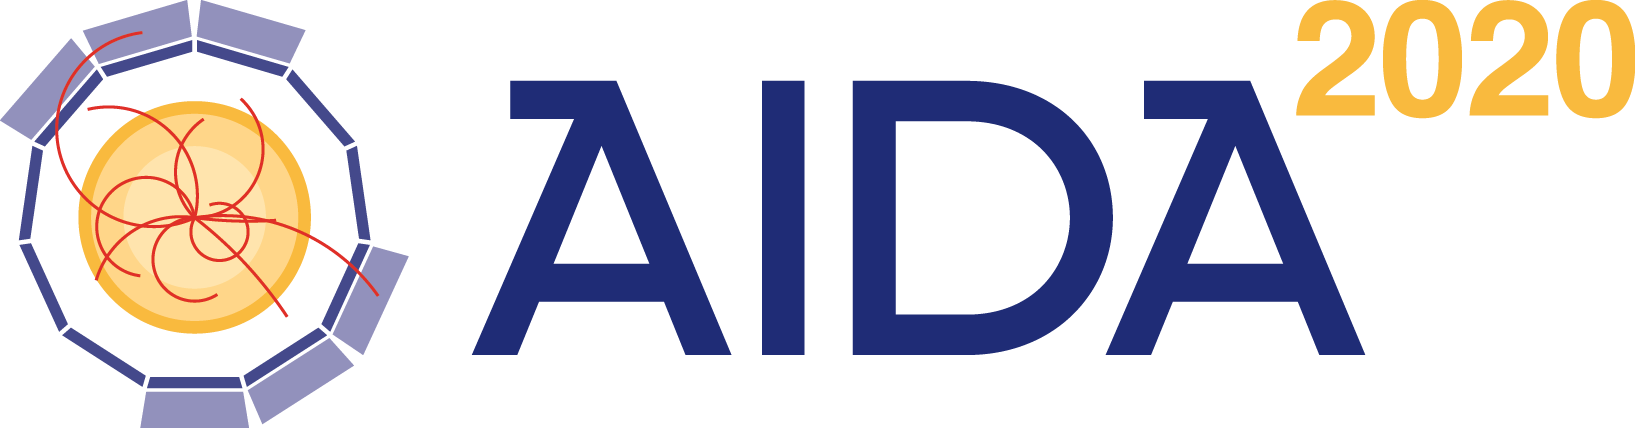
\includegraphics[height=25mm] {./setup/AIDA2020-logo}

\vspace{0.02cm}

{\sffamily{\underline{\hspace{6cm}Advanced European Infrastructures for Detectors at Accelerators}}}

\vspace{2cm}

\begin{center}
{\fontsize{72}{32}\selectfont{\bfseries{#1}}}

\vspace{3cm}
{\Huge\bf{#2}}
\vspace{3cm}
\begin{figure}[b]
  \begin{center}
    
\includegraphics[height=15mm] {./setup/Horizon2020-grant-logo}
  \end{center}
\end{figure}
\end{center}
}
\newcommand{\AIDAtitle}[3]{
\begin{titlepage}
\basictitle{#1}{#2}
\begin{center}
{#3}
\end{center}
\end{titlepage}
}

%
\pagestyle{fancyplain}{\fancyfoot[C]{\sffamily{DDG4 User Manual}}}
%
\begin{document}   
%
\mytitle{DDG4}   % Abbreviated title
{  % Detailed title
A Simulation Toolkit for \\
\vspace{0.5cm}
High Energy Physics Experiments\\
\vspace{0.5cm}
using Geant4 and the \\
\vspace{0.5cm}
DD4hep Geometry Description\\
}
{  % Author list
M. Frank \\
{CERN, 1211 Geneva 23, Switzerland}
}
%
%
%==  Abstract  ===============================================================
\pagestyle{plain}
\pagenumbering{Roman}
\setcounter{page}{1}
\begin{abstract}
%=============================================================================

\noindent
\normalsize
Simulating the detector response is an essential tool in high energy physics
to analyze the sensitivity of an experiment to the underlying physics.
Such simulation tools require a detailed though convenient detector description as 
it is provided by the \DDhep toolkit.
We will present the generic simulation toolkit \DDG using the \DDhep detector 
description toolkit. 
The toolkit implements a modular and flexible approach to simulation activities
using Geant4. User defined simulation applications using \DDG 
can easily be configured, extended using specialized action routines.
The design is strongly driven by easy of use;
developers of detector descriptions and applications using
them should provide minimal information and minimal specific
code to achieve the desired result.

\end{abstract}

\vspace{10cm}

\begin{center}
{\large{\bf{
\begin{tabular} {| l | l | l |}
\hline
\multicolumn{3}{| c |}{} \\[0.2cm]
\multicolumn{3}{| c |}{Document History} \\[0.2cm]
\multicolumn{3}{| c |}{} \\[0.2cm]
\hline
                 &      &        \\
Document         &      &        \\
version          & Date & Author \\[0.2cm] \hline
                 &      &        \\
1.0              & 19/11/2013 & Markus Frank CERN/LHCb  \\
                 &      &        \\        \hline 
\end{tabular}
}}}
\end{center}

\clearpage
%
%
%==  TOC  ====================================================================
\tableofcontents
\clearpage
%
%
%=============================================================================
% Manual
%=============================================================================
\pagenumbering{arabic}
\setcounter{page}{1}
\graphicspath{{./figs/}}

%=============================================================================
\section{Introduction}
\label{sec:ddg4-user-manual-introduction}
%=============================================================================
\noindent
This manual should introduce to the DDG4 framework. 
One goal of \DDG is to easily configure the simulation applications
capable of simulating the physics response of detector configurations 
as they are used for example in high energy physics experiments.
In such simulation programs the user normally has to define the 
experimental setup in terms of its geometry and in terms of its 
active elements which sample the detector response.

\noindent
The goal of \DDG is to generalize the configuration of a simulation
application to a degree, which does not force users to write code
to test a detector design. At the same time it should of course
be feasible to supply specialized user written modules which are supposed
to seamlessly operate together with standard modules supplied by the toolkit.
Detector-simulation depends strongly on the use of an underlying simulation
toolkit, the most prominent candidate nowadays being Geant4~\cite{bib:geant4}.
\DDhep supports simulation activities with Geant4 providing
an automatic translation mechanism between geometry representations.
The simulation response in the active elements of the detector
is strongly influenced by the technical 
choices and precise simulations depends on the very specific detection techniques.

\noindent
Similar to the aim of \DDhep\cite{bib:DD4hep}, 
where with time a standard palette of detector
components developed by users should become part of the toolkit,
\DDG also hopes to provide a standard palette of components used
to support simulation activities for detector layouts
where detector designers may base the simulation of a planned experiment 
on these predefined components for initial design and optimization 
studies. The longterm vision is to construct simulation applications
writing only new components not yet present i.e. the main work will be to
select the appropriate components from the palette and connect them
to a functional program.

\noindent
This is not a manual to Geant4 nor the basic infrastructure of \DDhep.
It is assumed that this knowledge is present and the typical glossary 
is known.

%=============================================================================
\section{The Geant4 User Interface}
\label{sec:ddg4-user-manual-geant4-interface}
%=============================================================================

\noindent
The Geant4 simulation toolkit~\cite{bib:geant4} implements a very complex
machinery to simulate the energy deposition of particles traversing materials.
To ease its usage for the clients and to shield clients from the complex
internals when actually implementing a simulation applications for a 
given detector design, it provides several user hooks
as shown in Figure~\ref{fig:ddg4-g4runmanager-anatomy}. Each of these hooks 
serves a well specialized purpose, but unfortunately also leads to very 
specialized applications. One aim of \DDG is to formalize these user 
actions so that the invocation at the appropriate time may be purely
data driven.
\begin{figure}[h]
  \begin{center}
    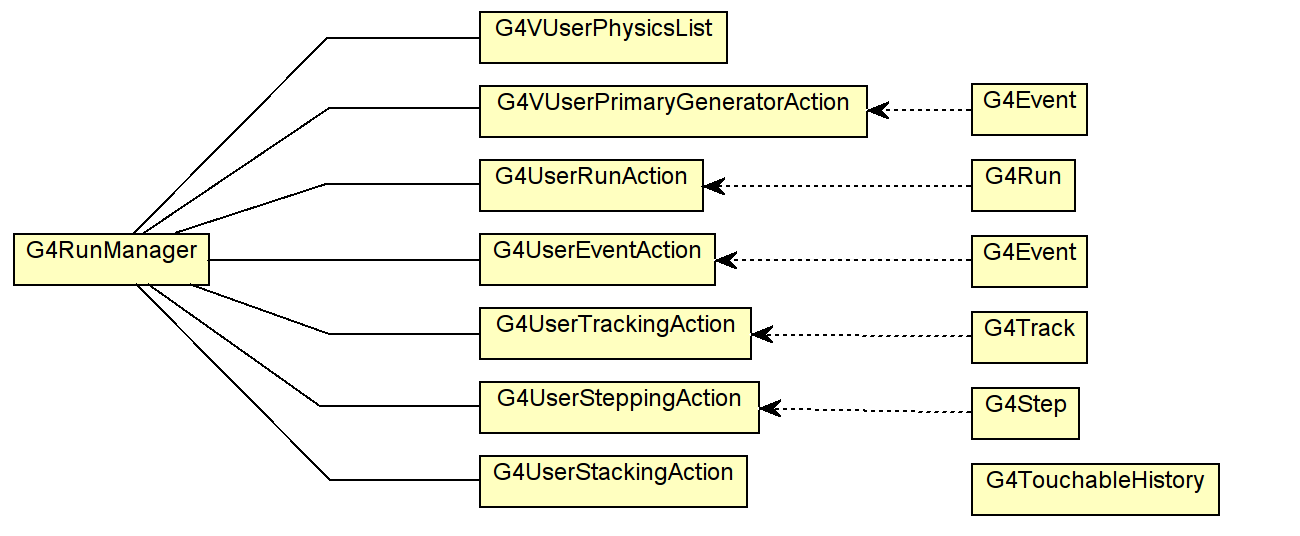
\includegraphics[height=70mm] {DDG4-G4RunManagerAnatomy}
    \caption{The various user hooks provided by Geant4. Not shown here
              is the callback system interfacing to the active elements
              of the detector design.}
    \label{fig:ddg4-g4runmanager-anatomy}
  \end{center}
\end{figure}

\noindent
In detail the following object-hooks allow the client to define user provided actions:
\begin{itemize}\itemcompact
\item The \bold{User Physics List} allows the client to customize and define 
    the underlying physics process(es) which define the particle interactions 
    inside the detector defined with the geometry description.
    These interactions define the detector response in terms of 
    energy depositions.
\item The \bold{Run Action} is called once at the start and end of a run. 
    i.e. a series of generated events. These two callbacks
    allow clients to define run-dependent actions such as statistics
    summaries etc.
\item The \bold{Primary Generator Action} is called for every event.
    During the callback all particles are created which form the 
    microscopic kinematic action of the particle collision.
    This input may either origin directly from an event generator program
    or come from file.
\item The \bold{Event Action} is called once at the start and the end of each event.
     It is typically used for a simple analysis of the processed event.
     If the simulated data should be written to some persistent medium, 
     the call at the end of the event processing is the appropriate place.
\item The \bold{Tracking Action} 
\item The \bold{Stepping Action} 
\item The \bold{Stacking Action} 
\end{itemize}
\noindent
Geant4 provides all callbacks with the necessary information in the form of 
appropriate arguments.

\noindent
Besides the callback system, Geant4 provides callbacks whenever a particle
traverses a sensitive volume. These callbacks are called 
- similar to event actions - once at the start and the end of the event,
but in addition, if either the energy deposit of a particle in the 
sensitive volume exceeds some threshold. The callbacks are formalized within 
the base class \tts{G4VSensitiveDetector}.


%=============================================================================
\section{DDG4 Implementation}
\label{sec:ddg4-user-manual-implementation}
%=============================================================================

\noindent
A basic design criteria of the a \DDG simulation application was to 
process any user defined hook provided by Geant4 as a series of algorithmic
procedures, which could be implemented either using inheritance or by 
a callback mechanism registering functions fulfilling a given signature.
Such sequences are provided for all actions mentioned in the list in 
Section~\ref{sec:ddg4-user-manual-geant4-interface} as well as for 
the callbacks to sensitive detectors.

\noindent
The callback mechanism was introduced to allow for weak coupling between 
the various actions. For example could an action performing monitoring
using histograms at the event level initialize or reset its histograms
at the start/end of each run. To do so, clearly a callback at the 
start/end of a run would be necessary.

\noindent
In the following sections a flexible and extensible interface to hooks
of Geant4 is discussed starting with the description of the basic
components \tts{Geant4Kernel} and \tts{Geant4Action} followed by the 
implementation of the relevant specializations.
The specializations exposed are sequences of such actions,
which also call registered objects.
In later section the configuration and the combination of these components 
forming a functional simulation application is presented.

%=============================================================================
\subsection{The Application Core Object: Geant4Kernel}
\label{sec:ddg4-user-manual-implementation-geant4kernel}
%=============================================================================

\noindent
The kernel object is the central context of a \DDG simulation application and
gives all clients access to the user hooks (see Figure~\ref{fig:ddg4-geant4-kernel}).
All Geant4 callback structures are exposed so that clients can easily 
objects implementing the required interface or register callbacks with the 
correct signature. Each of these action sequences is connected to an instance
of a Geant4 provided callback structure as it is shown in
Figure~\ref{fig:ddg4-g4runmanager-anatomy}.
\begin{figure}[h]
  \begin{center}
    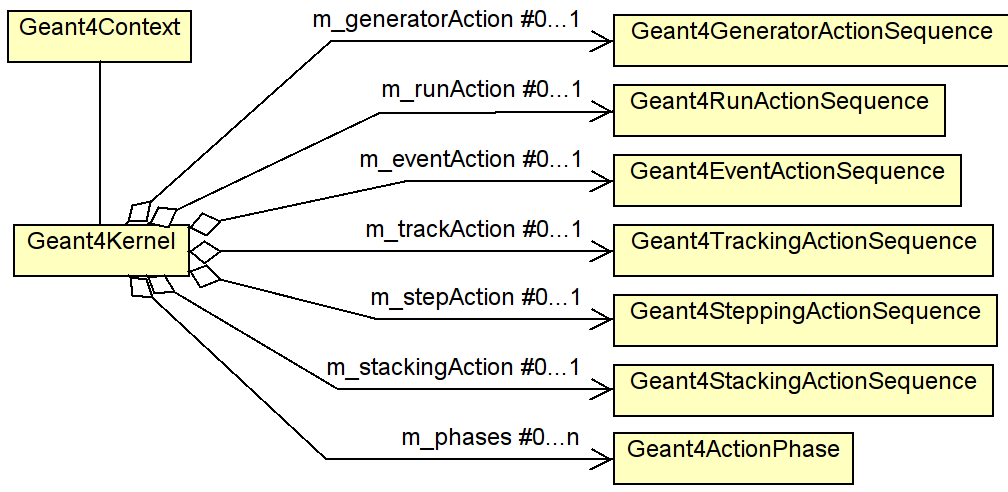
\includegraphics[height=65mm] {DDG4-Geant4Kernel}
    \caption{The main application object gives access to all sequencing actions
    in a \DDG4 application. Sequence actions are only container of user actions
    calling one user action after the other. Optionally single callbacks may 
    be registered to a user action.}
    \label{fig:ddg4-geant4-kernel}
  \end{center}
\end{figure}

%=============================================================================
\subsection{Action Sequences}
\label{sec:ddg4-user-manual-implementation-geant4action-sequences}
%=============================================================================

\noindent
As shown in 

%=============================================================================
\subsection{The Base Class of DDG4 Actions: Geant4Action}
\label{sec:ddg4-user-manual-implementation-geant4action-base}
%=============================================================================

\noindent
The class \tts{Geant4Action} is a common component interface providing 
the basic interface to the framework to
\begin{itemize}\itemcompact
\item configure the component using a property mechanism
\item provide an appropriate interface to Geant4 interactivity. The interactivity 
    included a generic way to change and access properties from the Geant4 UI 
    prompt as well as executing registered commands.
\item As shown in Figure~\ref{fig:ddg4-implementation-geant4-action}, the 
    base class also provides to its sub-class a reference to the \tts{Geant4Kernel}
    objects through the \tts{Geant4Context}.
\end{itemize}
The \tts{Geant4Action} is a named entity and can be uniquely identified within
a sequence attached to one Geant4 user callback.
%=============================================================================
\begin{figure}[h]
  \begin{center}
    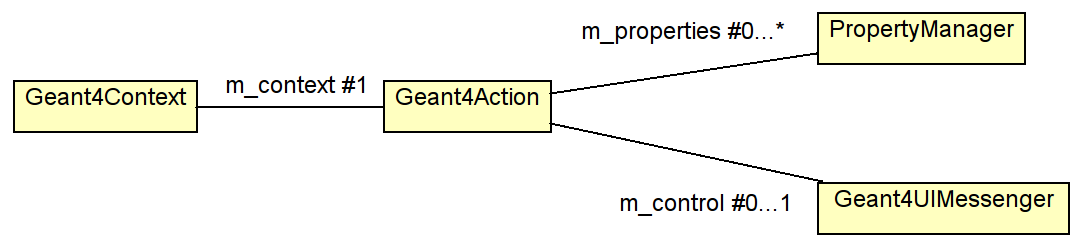
\includegraphics[height=30mm] {DDG4-Geant4Action}
    \caption{The design of the common base class \tts{Geant4Action}.}
    \label{fig:ddg4-implementation-geant4-action}
  \end{center}
\end{figure}

\noindent
\DDG knows two types of actions: global actions and anonymous actions.
Global actions are accessible externally from the \tts{Geant4Kernel} instance.
Global actions are also re-usable and hence may be contribute to several 
action sequences (see the following chapters for details). Global actions 
are uniquely identified by their name.
Anonymous actions are known only within one sequence and normally
are not shared between sequences.

%=============================================================================
\subsubsection{The Properties of \bold{Geant4Action} Instances}
\label{sec:ddg4-implementation-geant4-action-properties}
%=============================================================================

\noindent
Nearly any subclass of a \tts{Geant4Action} needs a flexible configuration 
in order to be reused, modified etc. The implementation of the mechanism
uses a very flexible value conversion mechanism using \tts{boost::spirit},
which support also conversions between unrelated types provided a dictionary 
is present.

\noindent
Properties are supposed to be member variables of a given action object.
To publish a property it needs to be declared in the constructor as shown here:
\begin{unnumberedcode}
  declareProperty("OutputLevel", m_outputLevel = INFO);
  declareProperty("Control",     m_needsControl = false);
\end{unnumberedcode}
The internal setup of the \tts{Geant4Action} objects then ensure that 
all declared properties will be set after the object construction to the 
values set in the setup file.

\noindent
\bold{Note:} Because the values can only be set \bold{after} the object 
was constructed, the actual values may not be used in the constructor
of any base or sub-class.

%=============================================================================
\subsection{Geant4 Action Sequences}
\label{sec:ddg4-user-manual-implementation-geant4action-sequences}
%=============================================================================

\noindent
All Geant4 user hooks are realized as action sequences. As shown in 
Figure~\ref{fig:ddg4-geant4-kernel} these sequences are accessible to the user,
who may attach specialized actions to the different action sequences. This 
allows a flexible handing of specialized user actions e.g. to dynamically
add monitoring actions filling histograms or to implement alternative hit 
creation mechanism in a sensitive detector for detailed detector studies.
Figure~\ref{fig:ddg4-implementation-sequence-calls} shows the schematic
call structure of an example {\tt{Geant4TrackingActionSequence}}:\\
\begin{figure}[h]
  \begin{center}
    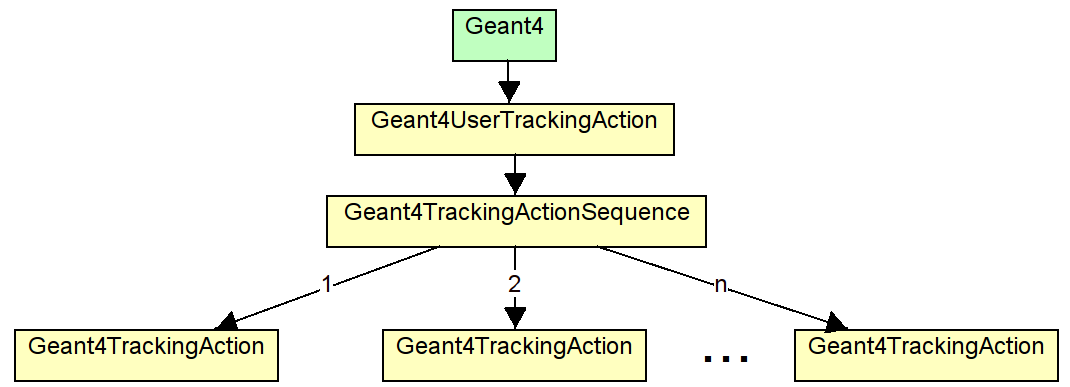
\includegraphics[width=150mm] {DDG4-TrackingActionCalls}
    \caption{The design of the tracking action sequence. Specialized 
               tracking action objects inherit from the \tts{Geant4TrackingAction}
               object and must be attached to the sequence.}
    \label{fig:ddg4-implementation-sequence-calls}
  \end{center}
\end{figure}

\noindent
Geant4 calls the function from the virtual interface (\tts{G4UserTrackingAction}), 
which is realised by the \tts{Geant4UserTrackingAction} with the single purpose to
propagate the call to the action sequence, which then calls all registered clients
of type \tts{Geant4TrackingAction}.

\noindent
The main action sequences have a fixed name. These are
\begin{itemize}

\item The \bold{RunAction} attached to the \tts{G4UserRunAction}, implemented 
    by the \tts{Geant4RunActionSequence} class and is called at the start and the end of 
    every run (beamOn). Members of the \tts{Geant4RunActionSequence} are of type
    \tts{Geant4RunAction} and receive the callbacks by overloading the two routines:
\begin{unnumberedcode}
/// begin-of-run callback
virtual void begin(const G4Run* run);
/// End-of-run callback
virtual void end(const G4Run* run);
\end{unnumberedcode}
    or register a callback with the signature {\tts{void (T::*)(const G4Run*)}}
    either to receive begin-of-run or end-or-calls using the methods:
\begin{unnumberedcode}
/// Register begin-of-run callback. Types Q and T must be polymorph!
template <typename Q, typename T> void callAtBegin(Q* p, void (T::*f)(const G4Run*));
/// Register end-of-run callback. Types Q and T must be polymorph!
template <typename Q, typename T> void callAtEnd(Q* p, void (T::*f)(const G4Run*));
\end{unnumberedcode}
    of the \tts{Geant4RunActionSequence} from the \tts{Geant4Context} object.


\item The \bold{EventAction} attached to the \tts{G4UserEventAction}, implemented 
    by the \tts{EventActionSequence} class and is called at the start and the end of 
    every event. Members of the \tts{Geant4EventActionSequence} are of type
    \tts{Geant4EventAction} and receive the callbacks by overloading the two routines:
\begin{unnumberedcode}
/// Begin-of-event callback
virtual void begin(const G4Event* event);
/// End-of-event callback
virtual void end(const G4Event* event);
\end{unnumberedcode}
    or register a callback with the signature {\tts{void (T::*)(const G4Event*)}}
    either to receive begin-of-run or end-or-calls using the methods:
\begin{unnumberedcode}
/// Register begin-of-event callback
template <typename Q, typename T> void callAtBegin(Q* p, void (T::*f)(const G4Event*));
/// Register end-of-event callback
template <typename Q, typename T> void callAtEnd(Q* p, void (T::*f)(const G4Event*));
\end{unnumberedcode}
    of the \tts{Geant4EventActionSequence} from the \tts{Geant4Context} object.


\item The \bold{GeneratorAction} attached to the \tts{G4VUserPrimaryGeneratorAction}, implemented 
    by the \tts{Geant4GeneratorActionSequence} class and is called at the start of 
    every event and provided all initial tracks from the Monte-Carlo generator.
    Members of the \tts{Geant4GeneratorActionSequence} are of type
    \tts{Geant4EventAction} and receive the callbacks by overloading the member function:
\begin{unnumberedcode}
/// Callback to generate primary particles
virtual void operator()(G4Event* event);
\end{unnumberedcode}
    or register a callback with the signature {\tts{void (T::*)(G4Event*)}}
    to receive calls using the method:
\begin{unnumberedcode}
/// Register primary particle generation callback.
template <typename Q, typename T> void call(Q* p, void (T::*f)(G4Event*));
\end{unnumberedcode}
    of the \tts{Geant4GeneratorActionSequence} from the \tts{Geant4Context} object.

\end{itemize}
\begin{figure}[t]
  \begin{center}
    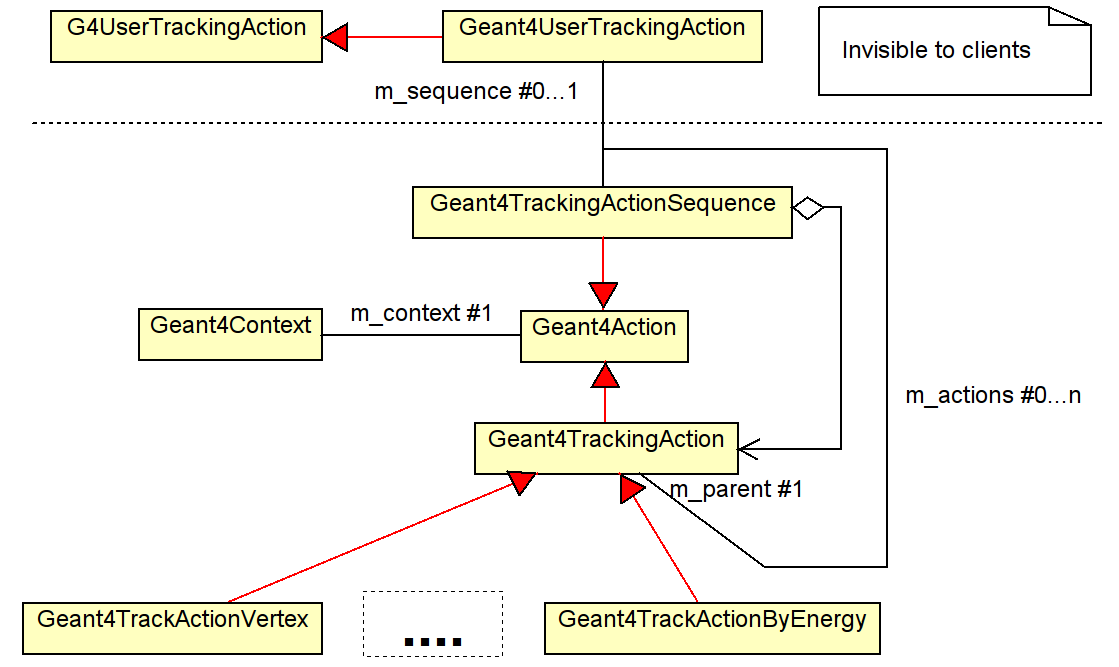
\includegraphics[width=160mm] {DDG4-TrackingAction}
    \caption{The design of the tracking action sequence. Specialized 
               tracking action objects inherit from the \tts{Geant4TrackingAction}
               object and must be attached to the sequence.}
    \label{fig:ddg4-implementation-tracking-action}
  \end{center}
\end{figure}

\begin{itemize}
\item The \bold{TrackingAction} attached to the \tts{G4UserTrackingAction}, 
    implemented by the \tts{Geant4-} \tts{Tracking\-Action\-Sequence} class 
    and is called at the start and the end of tracking one single particle 
    trace through the material of the detector.
    Members of the \tts{Geant4\-Tracking\-ActionSequence} are of type
    \tts{Geant4TrackingAction} and receive the callbacks by overloading the member function:
\begin{unnumberedcode}
/// Pre-tracking action callback
virtual void begin(const G4Track* trk);
/// Post-tracking action callback
virtual void end(const G4Track* trk);
\end{unnumberedcode}
    or register a callback with the signature {\tts{void (T::*)(const G4Step*, G4SteppingManager*)}}
    to receive calls using the method:
\begin{unnumberedcode}
/// Register Pre-track action callback
template <typename Q, typename T> void callAtBegin(Q* p, void (T::*f)(const G4Track*));
/// Register Post-track action callback
template <typename Q, typename T> void callAtEnd(Q* p, void (T::*f)(const G4Track*));
\end{unnumberedcode}
Figure~\ref{fig:ddg4-implementation-tracking-action} show as an example 
the design (class-diagram) of the \tts{Geant4TrackingAction}.


\item The \bold{SteppingAction} attached to the \tts{G4UserSteppingAction}, implemented 
    by the \tts{Geant4-} \tts{SteppingActionSequence} class and is called for each
    step when tracking a particle.
    Members of the \tts{Geant4SteppingActionSequence} are of type
    \tts{Geant4SteppingAction} and receive the callbacks by overloading the member function:
\begin{unnumberedcode}
/// User stepping callback
virtual void operator()(const G4Step* step, G4SteppingManager* mgr);
\end{unnumberedcode}
    or register a callback with the signature {\tts{void (T::*)(const G4Step*, G4SteppingManager*)}}
    to receive calls using the method:
\begin{unnumberedcode}
/// Register stepping action callback.
template <typename Q, typename T> void call(Q* p, void (T::*f)(const G4Step*, 
                                                               G4SteppingManager*));
\end{unnumberedcode}


\item The \bold{StackingAction} attached to the 
    {\tts{G4UserStackingAction}}, implemented by the \tts{Geant4-}\\
    \tts{StackingActionSequence} class.
    Members of the \tts{Geant4StackingActionSequence} are of type\\
    \detdesc{html/class_d_d4hep_1_1_simulation_1_1_geant4_stacking_action.html}
    {\tts{Geant4StackingAction}} and receive the callbacks by overloading the member functions:
\begin{unnumberedcode}
/// New-stage callback
virtual void newStage();
/// Preparation callback
virtual void prepare();
\end{unnumberedcode}
    or register a callback with the signature {\tts{void (T::*)()}}
    to receive calls using the method:
\begin{unnumberedcode}
/// Register begin-of-event callback. Types Q and T must be polymorph!
template <typename T> void callAtNewStage(T* p, void (T::*f)());
/// Register end-of-event callback. Types Q and T must be polymorph!
template <typename T> void callAtPrepare(T* p, void (T::*f)());
\end{unnumberedcode}
\end{itemize}

\noindent
All sequence types support the method \tts{void adopt(T* member\_reference)}
to add the members. Once adopted, the sequence takes ownership and manages
the member. The design of all sequences is very similar. 

%=============================================================================
\subsection{Sensitive Detectors}
\label{sec:ddg4-user-manual-geant4sensitivedetectors}
%=============================================================================

\noindent
Sensitive detectors are associated by the detector designers to all active 
materials, which would produce a signal which can be read out. In Geant4 this concept
is realized by using a base class \tts{G4VSensitiveDetector}.
The mandate of a sensitive detector is the construction of hit objects 
using information from steps along a particle track. 
The \tts{G4VSensitiveDetector} receives 
a callback at the begin and the end of the event processing and at each step
inside the active material whenever an energy deposition occurred.

\begin{figure}[t]
  \begin{center}
    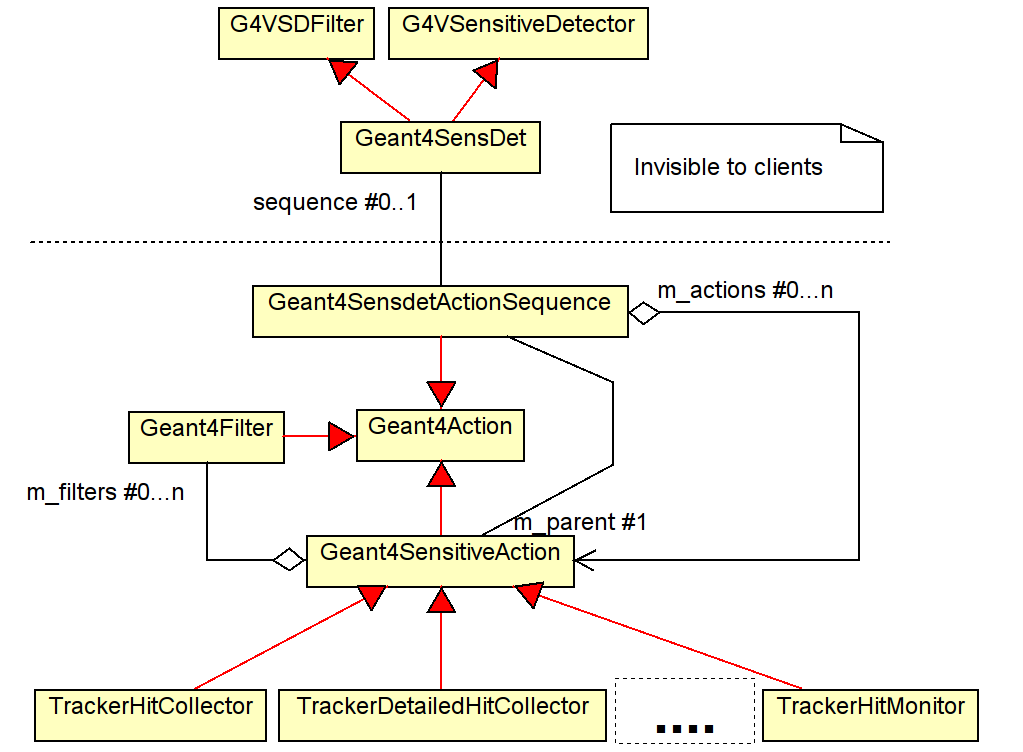
\includegraphics[height=110mm] {DDG4-Sensitive-detector}
    \caption{The sensitive detector design. The actual energy deposits are 
        collected in user defined subclasses of the \tts{Geant4Sensitive}.
        Here, as an example possible actions called \tts{TrackerHitCollector},
        \tts{TrackerDetailedHitCollector} and \tts{TrackerHitMonitor} are shown.}
    \label{fig:ddg4-implementation-sensitive-detector}
  \end{center}
\end{figure}

\noindent
The sensitive actions do not necessarily deal only the collection of energy 
deposits, but could also be used to simply monitor the performance of the
active element e.g. by producing histograms of the absolute value or the 
spacial distribution of the depositions.

\noindent
Within \DDG the concept of sensitive  detectors is implemented as a
configurable  action sequence of type 
\detdesc{html/class_d_d4hep_1_1_simulation_1_1_geant4_sens_det_action_sequence.html}
{\tts{Geant4SensDetActionSequence}}
calling members of the type 
\detdesc{html/struct_d_d4hep_1_1_simulation_1_1_geant4_sensitive.html}
{\tts{Geant4Sensitive}} as shown in 
Figure~\ref{fig:ddg4-implementation-sensitive-detector}. The actual processing
part of such a sensitive action is only called if the and of a set of
required filters of type \tts{Geant4Filter} is positive (see also 
section~\ref{sec:ddg4-implementation-sensitive-detector-filters}). No filter 
is also positive. Possible filters are e.g. particle filters, which ignore the
sensitive detector action if the particle is a \tts{geantino} or if the
energy deposit is below a given threshold.

\noindent
Objects of type \tts{Geant4Sensitive} receive the callbacks by overloading the 
member function:
\begin{unnumberedcode}
  /// Method invoked at the beginning of each event.
  virtual void begin(G4HCofThisEvent* hce);
  /// Method invoked at the end of each event.
  virtual void end(G4HCofThisEvent* hce);
  /// Method for generating hit(s) using the information of G4Step object.
  virtual bool process(G4Step* step, G4TouchableHistory* history);
  /// Method invoked if the event was aborted.
  virtual void clear(G4HCofThisEvent* hce);
\end{unnumberedcode}
or register a callback with the signature {\tts{void (T::*)(G4HCofThisEvent*)}}
respectively {\tts{void (T::*)(G4Step*, G4TouchableHistory*)}} 
to receive callbacks using the methods:
\begin{unnumberedcode}
  /// Register begin-of-event callback
  template <typename T> void callAtBegin(T* p, void (T::*f)(G4HCofThisEvent*));
  /// Register end-of-event callback
  template <typename T> void callAtEnd(T* p, void (T::*f)(G4HCofThisEvent*));
  /// Register process-hit callback
  template <typename T> void callAtProcess(T* p, void (T::*f)(G4Step*, G4TouchableHistory*));
  /// Register clear callback
  template <typename T> void callAtClear(T* p, void (T::*f)(G4HCofThisEvent*));
\end{unnumberedcode}
Please refer to the Geant4 Applications manual from the Geant4 web page for 
further details about the concept of sensitive detectors.

%=============================================================================
\subsubsection{Helpers of Sensitive Detectors: The Geant4VolumeManager}
\label{sec:ddg4-user-manual-geant4volumemanager}%=============================================================================

\noindent
Sooner or later, when a hit is created in a sensitive placed volume, the
hit must be associated with this volume. For this purpose \DDhep provides 
the concept of the \tts{VolumeManager}, which identifies placed volumes uniquely 
by a 64-bit identifier, the $CellID$. This mechanism allows to quickly
retrieve a given volume given the hit data containing the $CellID$.
The $CellID$ is a very compressed representation for any element in the 
hierarchy of placed volumes to the sensitive volume in question.

\noindent 
During the simulation the reverse mechanism must be applied: Geant4 provides
the hierarchy of \tts{G4PhysicalVolumes} to the hit location and the local coordinates
of the hit within the sensitive volume. Hence to determine the volume identifier
is essential to store hits so that they can be later accessed and processed efficiently.
This mechanism is provided by the \tts{Geant4VolumeManager}. Clients typically do not
interact with this object, any access necessary is provided by the
\tts{Geant4Sensitive} action:
\begin{unnumberedcode}
  /// Method for generating hit(s) using the information of G4Step object.
  bool MySensitiveAction:process(G4Step* step,G4TouchableHistory* /*hist*/ ) {
    ...
    Hit* hit = new Hit();
    // *** Retrieve the cellID  ***
    hit->cellID = cellID(step);
    ...
  }
\end{unnumberedcode}
The call is realized using a member function provided by the 
\tts{Geant4Sensitive} action:
\begin{unnumberedcode}
  /// Returns the cellID of the sensitive volume corresponding to the step
  /** The CellID is the VolumeID + the local coordinates of the sensitive area.
   *  Calculated by combining the VolIDS of the complete geometry path (Geant4TouchableHistory)
   *  from the current sensitive volume to the world volume
   */
  long long int cellID(G4Step* step);
\end{unnumberedcode}

\noindent
\bold{Note:}\\
The \tts{Geant4VolumeManager} functionality is not for free! It requires that


\noindent
-- match Geant4 volume with TGeo volume

%=============================================================================
\subsubsection{DDG4 Intrinsic Sensitive Detectors}
%=============================================================================
\noindent
Currently there are two generic sensitive detectors implemented in DDG4:
\begin{itemize}\itemcompact
\item The \tts{Geant4TrackerAction}, which may be used to handle tracking devices.
  This sensitive detector produces one hit for every energy deposition of Geant4
  i.e. for every callback to 
\begin{unnumberedcode}
  /// Method for generating hit(s) using the information of G4Step object.
  virtual bool process(G4Step* step, G4TouchableHistory* history);
\end{unnumberedcode}
  See the implementation file 
  \detdesc{html/_geant4_s_d_actions_8cpp_source.html}{DDG4/plugins/Geant4SDAction.cpp}
  for details. The produced hits are of type 
  \detdesc{html/_geant4_data_8h_source.html}{Geant4Tracker::Hit}.

\item The \tts{Geant4CalorimeterAction}, which may be used to handle 
  generic calorimeter like devices.
  This sensitive detector produces at most one hit for every cell in the calorimeter.
  If several tracks contribute to the energy deposit of this cell, the contributions
  are added up.
  See the implementation file 
  \detdesc{html/_geant4_s_d_actions_8cpp_source.html}{DDG4/plugins/Geant4SDAction.cpp}
  for details. The produced hits are of type 
  \detdesc{html/_geant4_data_8h_source.html}{Geant4Calorimeter::Hit}.
  propagate the MC truth information with respect to each track kept in the 
  particle record.
\end{itemize}

\noindent
Both sensitive detectors use the \tts{Geant4VolumeManager} discussed in 
section~\ref{sec:ddg4-user-manual-geant4volumemanager} to identify the sensitive elements.

\noindent
\bold{PLEASE NOTE:}\\
The above palette of generic sensitive detectors only contains two very
often used implementations. We hope, that this palette over time grows from
external contributions of other generic sensitive detectors. We would be happy 
to extend this palette with other generic implementations. One example would
be the handling of the simulation response for optical detectors like RICH-Cerenkov
detectors.

%=============================================================================
\subsubsection{Sensitive Detector Filters}
\label{sec:ddg4-implementation-sensitive-detector-filters}
%=============================================================================

\noindent
The concept of filters allows to build more flexible sensitive detectors by
restricting the hit processing of a given instance of a sensitive action.

\begin{itemize}\itemcompact
\item Examples would be to demand a given particle type before a sensitive action is 
invoked: a sensitive action dealing with optical photons (RICH detectors, etc),
would e.g. not be interested in energy depositions of other particles.
A filter object restricting the particle type to optical photons would 
be appropriate.
\item Another example would be to implement a special action instance, which would
be only called if the filter requires a minimum energy deposit.
\end{itemize}
There are plenty of possible applications, hence we would like 
to introduce this feature here.

\noindent
Filters are called by Geant4 before the
hit processing in the sensitive detectors start. The global filters
may be shared between many sensitive detectors. Alternatively filters
may be directly attached to the sensitive detector in question.
Attributes are directly passed as properties to the filter action.

\noindent
Technically do \tts{Geant4Filter} objects inherit from the base class
\tts{Geant4Filter} (see Figure~\ref{fig:ddg4-implementation-sensitive-detector-filters}.
Any filter inherits from the common base class \tts{Geant4Filter}, then 
several specializations may be configured like filters to select/reject 
particles, to specify the minimal energy deposit to be processed etc.
A sensitive detector is called if the filter callback with the signature
returns a true result:
\begin{unnumberedcode}
  /// Filter action. Return true if hits should be processed
  virtual bool operator()(const G4Step* step) const;
\end{unnumberedcode}
\begin{figure}[h]
  \begin{center}
    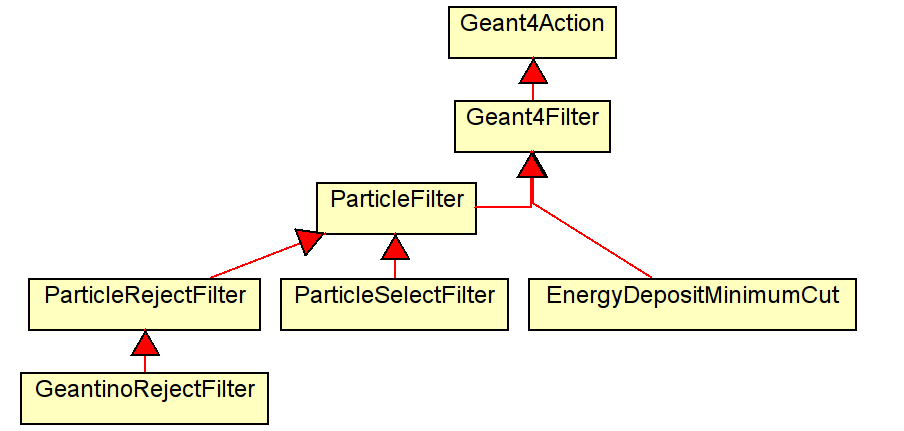
\includegraphics[height=65mm] {DDG4-SensitiveFilterClasses}
    \caption{The sensitive detector filters design. The shown class
        diagram is actually implemented.}
    \label{fig:ddg4-implementation-sensitive-detector-filters}
  \end{center}
\end{figure}

\newpage

%=============================================================================
\subsection{The Geant4 Physics List}
\label{sec:ddg4-implementation-physics-list}
%=============================================================================
\noindent 
Geant4 provides the base class \tts{G4VUserPhysicsList}, which allows users
to implement customized physics according to the studies to be made.
Any user defined physics list must provide this interface. DDG4 provides such an interface
through the ROOT plugin mechanism using the class \tts{G4VModularPhysicsList}.
The flexibility of \DDG allows for several possibilities to setup the Geant4
physics list. Instead of explicitly coding the physics list, \DDG foresees the
usage of the plugin mechanism to instantiate the necessary calls to Geant4 in a
sequence of actions:
\begin{itemize}
\item The \bold{physics list} is realized as a sequence of actions of type 
    \detdesc{html/class_d_d4hep_1_1_simulation_1_1_geant4_physics_list_action_sequence.html}
    {\tts{Geant4PhysicsListActionSequence}}.
    Members of the \detdesc{html/class_d_d4hep_1_1_simulation_1_1_geant4_physics_list_action_sequence.html}
    {\tts{Geant4PhysicsListActionSequence}} are of type
    \detdesc{html/class_d_d4hep_1_1_simulation_1_1_geant4_physics_list.html}
    {\tts{Geant4PhysicsList}} and receive the callbacks by overloading 
    the member functions:
\begin{unnumberedcode}
  /// Callback to construct the physics constructors
  virtual void constructProcess(Geant4UserPhysics* interface);
  /// constructParticle callback
  virtual void constructParticles(Geant4UserPhysics* particle);
  /// constructPhysics callback
  virtual void constructPhysics(Geant4UserPhysics* physics);
\end{unnumberedcode}
    or register a callback with the signature {\tts{void (T::*)(Geant4UserPhysics*)}}
    to receive calls using the method:
\begin{unnumberedcode}
  /// Register process construction callback t
  template <typename Q, typename T> void constructProcess(Q* p, void (T::*f)(Geant4UserPhysics*));
  /// Register particle construction callback
  template <typename Q, typename T> void constructParticle(Q* p, void (T::*f)(Geant4UserPhysics*));
\end{unnumberedcode}
    The argument of type \detdesc{html/class_d_d4hep_1_1_simulation_1_1_geant4_user_physics.html}
    {\tts{Geant4UserPhysics}} provides a basic interface to the original
    \tts{G4VModular}- \tts{PhysicsList}, which allows to register physics constructors etc.

\item In most of the cases the above approach is an overkill and often even too flexible.
    Hence, alternatively, the physics list may consist of a single entry of type 
    \detdesc{html/class_d_d4hep_1_1_simulation_1_1_geant4_physics_list.html}
    {\tts{Geant4PhysicsList}}.
\end{itemize}

\noindent
The basic implementation of the \tts{Geant4PhysicsList} supports the usage of various
\begin{itemize}\itemcompact
\item \detdesc{html/_geant4_particles_8cpp_source.html}{particle constructors}, 
    such as single particle constructors like   
    \tts{G4Gamma} or \tts{G4Proton}, or whole particle groups like
    \tts{G4BosonConstructor} or \tts{G4IonConstrutor},
\item \detdesc{html/_geant4_processes_8cpp_source.html}{physics process constructors}, 
    such as e.g. \tts{G4GammaConversion},
    \tts{G4PhotoElectricEffect} or\\ \tts{G4ComptonScattering}, 
\item \detdesc{html/_geant4_physics_constructors_8cpp_source.html}{physics constructors} 
    combining particles and the corresponding 
    interactions, such as\\ e.g. \tts{G4OpticalPhysics},
    \tts{HadronPhysicsLHEP} or \tts{G4HadronElasticPhysics} and
\item \detdesc{html/_geant4_particles_8cpp_source.html}{predefined Geant4 physics lists}, 
    such as \tts{FTFP\_BERT},
    \tts{CHIPS} or \tts{QGSP\_INCLXX}. This option is triggered by the 
    content of the string property "extends" of the \tts{Geant4Kernel::physicsList()} action.
\end{itemize}
These constructors are internally connected to the above callbacks to register themselves. 
The constructors are instantiated using the ROOT plugin mechanism.

\noindent
The description of the above interface is only for completeness. The basic idea is,
that the physics list with its particle and physics constructors is configured
entirely data driven using the setup mechanism described in the following
chapter. However, DDG4 is not limited to the data driven approach. Specialized 
physics lists may be supplied, but there should be no need.
New physics lists could always be composed by actually providing new physics
constructors and actually publishing these using the factory methods:
\begin{code}
// Framework include files
#include "DDG4/Factories.h"

#include "My_Very_Own_Physics_Constructor.h"
DECLARE_GEANT4_PHYSICS(My_Very_Own_Physics_Constructor)
\end{code}
where \tts{My\_Very\_Own\_Physics\_Constructor} represents a sub-class of
\tts{G4VPhysicsConstructor}.

\newpage
%=============================================================================
\subsection{The Support of the Geant4 UI: \tts{Geant4UIMessenger}}
\label{sec:ddg4-user-manual-geant4action-base}
%=============================================================================

\noindent
The support of interactivity in Geant4 is mandatory to debug detector
setups in small steps. The Geant4 toolkit did provide for this reason 
a machinery of UI commands.
\begin{figure}[h]
  \begin{center}
    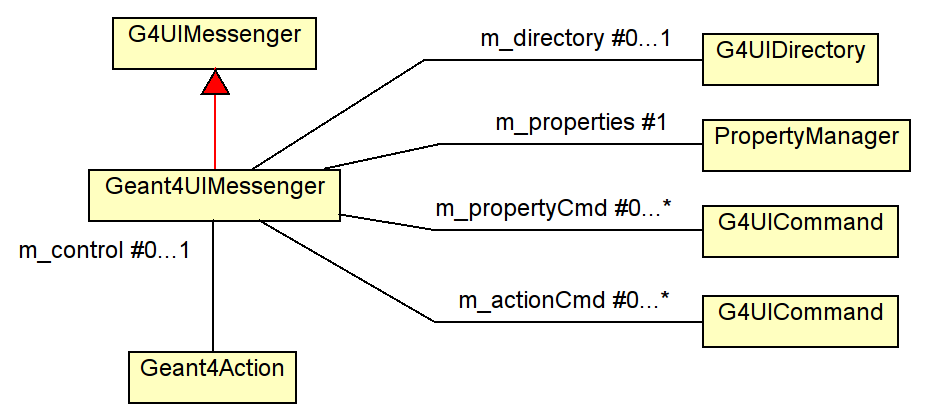
\includegraphics[height=70mm] {DDG4-UIMessenger}
    \caption{The design of the \tts{Geant4UIMessenger} class responsible for
        the interaction between the user and the components of \DDG and Geant4.}
    \label{fig:ddg4-tracking-action}
  \end{center}
\end{figure}

\noindent
The UI control is enabled, as soon as the property "Control" (boolean) is set to true.
Be default all properties of the action are exported.
Similar to the callback mechanism described above it is also feasible to
register any object callback invoking a method of a \tts{Geant4Action}-subclass. 

\noindent
The following (shortened) screen dump illustrates the usage of the 
generic interface any Geant4Action offers:
\begin{unnumberedcode}
Idle> ls
Command directory path : /
 Sub-directories : 
   /control/   UI control commands.
   /units/   Available units.
   /process/   Process Table control commands.
   /ddg4/   Control for all named Geant4 actions
   ...
Idle> cd /ddg4
Idle> ls
...
Control for all named Geant4 actions

 Sub-directories : 
   /ddg4/RunInit/   Control hierarchy for Geant4 action:RunInit
   /ddg4/RunAction/   Control hierarchy for Geant4 action:RunAction
   /ddg4/EventAction/   Control hierarchy for Geant4 action:EventAction
   /ddg4/GeneratorAction/   Control hierarchy for Geant4 action:GeneratorAction
   /ddg4/LCIO1/   Control hierarchy for Geant4 action:LCIO1
   /ddg4/Smear1/   Control hierarchy for Geant4 action:Smear1
   /ddg4/PrimaryHandler/   Control hierarchy for Geant4 action:PrimaryHandler
   /ddg4/TrackingAction/   Control hierarchy for Geant4 action:TrackingAction
   /ddg4/SteppingAction/   Control hierarchy for Geant4 action:SteppingAction
   /ddg4/ParticleHandler/   Control hierarchy for Geant4 action:ParticleHandler
   /ddg4/UserParticleHandler/   Control hierarchy for Geant4 action:UserParticleHandler
   ...
Idle> ls Smear1
Command directory path : /ddg4/Smear1/
 ...
 Commands : 
   show * Show all properties of Geant4 component:Smear1
   Control * Property item of type bool
   Mask * Property item of type int
   Name * Property item of type std::string
   Offset * Property item of type ROOT::Math::LorentzVector<ROOT::Math::PxPyPzE4D<double> >
   OutputLevel * Property item of type int
   Sigma * Property item of type ROOT::Math::LorentzVector<ROOT::Math::PxPyPzE4D<double> >
   name * Property item of type std::string
Idle> Smear1/show
PropertyManager: Property Control = True
PropertyManager: Property Mask = 1
PropertyManager: Property Name = 'Smear1'
PropertyManager: Property Offset = ( -20 , -10 , -10 , 0 )
PropertyManager: Property OutputLevel = 4
PropertyManager: Property Sigma = ( 12 , 8 , 8 , 0 )
PropertyManager: Property name = 'Smear1'

Idle> Smear1/Offset (200*mm, -3*mm, 15*mm, 10*ns)
Geant4UIMessenger: +++ Smear1> Setting property value Offset = (200*mm, -3*mm, 15*mm, 10*ns)  
                               native:( 200 , -3 , 15 , 10 ).
Idle> Smear1/show                                
...
PropertyManager: Property Offset = ( 200 , -3 , 15 , 10 )

\end{unnumberedcode}

\newpage


%=============================================================================
\section{Setting up DDG4}
\label{sec:ddg4-implementation-setup}
%=============================================================================

\noindent
\DDG offers several possibilities to configure a simulation application
using
\begin{itemize}\itemcompact
\item XML files,
\item by coding a setup script loaded from the \tts{ROOT} interpreter 
	with the AClick	mechanism.
\item by creating a setup script using \tts{python} and 
	\tts{ROOT}'s reflection mechanism exposed by \tts{PyROOT}.
\end{itemize}
The following subsection describe these different mechanism. An attempt was made
to match the naming conventions of all approaches where possible.

%=============================================================================
\subsection{Setting up DDG4 using XML}
\label{sec:ddg4-implementation-setup-xml}
%=============================================================================

\noindent
A special plugin was developed to enable the configuration of \DDG using
XML structures. These files are parsed identically to the geometry setup
in \DDhep the only difference is the name of the root-element, which for 
\DDG is \tts{<geant4\_setup>}. 
The following code snippet shows the basic structure of a \DDG setup file:
\begin{unnumberedcode}
<geant4_setup>
  <physicslist>          ,,,  </physicslist>  <!-- Definition of the physics list          -->
  <actions>              ...  </actions>      <!-- The list of global actions              -->
  <phases>               ...  </phases>       <!-- The definition of the various phases    -->
  <filters>              ...  </filters>      <!-- The list of global filter actions       -->
  <sequences>            ...  </sequences>    <!-- The list of defined sequences           -->
  <sensitive_detectors>  ...  </sensitive_detectors>  <!-- The list of sensitive detectors -->
  <properties>           ...  </properties>   <!-- Free format option sequences            -->
</geant4_setup>
\end{unnumberedcode}
To setup a \DDG4 application any number of xml setup files may be interpreted 
iteratively. In the following subsections the content of these first level sub-trees will
be discussed.

%=============================================================================
\subsubsection{Setup of the Physics List}
\label{sec:ddg4-setup-xml-physicslist}
%=============================================================================

\noindent
The main tag to setup a physics list is \tts{<physicslist>} with the 
\tts{name} attribute defining the instance of the \tts{Geant4PhysicsList} object.
An example code snippet is shown below in Figure~\ref{fig:ddg4-setup-xml-physicslist}.

\begin{code}
<geant4_setup>
  <physicslist name="Geant4PhysicsList/MyPhysics.0">

    <extends name="QGSP_BERT"/>                    <!-- Geant4 basic Physics list -->

    <particles>                                    <!-- Particle constructors     -->
      <construct name="G4Geantino"/>
      <construct name="G4ChargedGeantino"/>
      <construct name="G4Electron"/>
      <construct name="G4Gamma"/>
      <construct name="G4BosonConstructor"/>
      <construct name="G4LeptonConstructor"/>
      <construct name="G4MesonConstructor"/>
      <construct name="G4BaryonConstructor"/>
      ...
    </particles>

    <processes>                                    <!-- Process constructors      -->
      <particle name="e[+-]" cut="1*mm">
        <process name="G4eMultipleScattering"  ordAtRestDoIt="-1"       ordAlongSteptDoIt="1"
                                               ordPostStepDoIt="1"/>
        <process name="G4eIonisation"          ordAtRestDoIt="-1"       ordAlongSteptDoIt="2"
                                               ordPostStepDoIt="2"/>
      </particle>
      <particle name="mu[+-]">
        <process name="G4MuMultipleScattering" ordAtRestDoIt="-1"       ordAlongSteptDoIt="1"     
                                               ordPostStepDoIt="1"/>
        <process name="G4MuIonisation"         ordAtRestDoIt="-1"       ordAlongSteptDoIt="2"
                                               ordPostStepDoIt="2"/>
      </particle>
      ...
    </processes>

    <physics>                                      <!-- Physics constructors      -->
      <construct name="G4EmStandardPhysics"/>
      <construct name="HadronPhysicsQGSP"/>
      ...
    </physics>
    
  </physicslist>
</geant4_setup>
\end{code}
\begin{figure}[h]
\caption{XML snippet showing the configuration of a physics list.}
\label{fig:ddg4-setup-xml-physicslist}
\end{figure}

\begin{itemize}\itemcompact
\item To base all these constructs on an already existing predefined Geant4 physics list
    use the \tts{<extends>} tag with the attribute containing the name of the physics list
    as shown in line 4.
\item To trigger a call to a \bold{particle constructors} (line 7-14), use the \tts{<particles>} section 
    and define the Geant4 particle constructor to be called by name. To trigger a call to
\item \bold{physics process constructors}, as shown in line 19-30, 
    Define for each particle matching the name pattern (regular expression!) and the 
    default cut value for the corresponding processes. The attributes ordXXXX correspond
    to the arguments of the Geant4 call \\
    \tts{G4ProcessManager::AddProcess(process,ordAtRestDoIt, ordAlongSteptDoIt,ordPostStepDoIt);}
    The processes themself are created using the ROOT plugin mechanism.
    To trigger a call to
\item \bold{physics constructors}, as shown in line 34-35, use the \tts{<physics>} section.
\end{itemize}
If only a predefined physics list is used, which probably already satisfies very many use cases,
all these section collapse to:
\begin{code}
<geant4_setup>
  <physicslist name="Geant4PhysicsList/MyPhysics.0">
    <extends name="QGSP_BERT"/>                    <!-- Geant4 basic Physics list -->
  </physicslist>
</geant4_setup>
\end{code}

%=============================================================================
\subsubsection{Setup of Global Geant4 Actions}
\label{sec:ddg4-setup-xml-geant4-actions}
%=============================================================================

\noindent
Global actions must be defined in the \tts{<actions>} section as shown in the following snippet:
\begin{code}
<geant4_setup>
  <actions>
    <action name="Geant4TestRunAction/RunInit">
      <properties Property_int="12345"
          Property_double="-5e15"
          Property_string="Startrun: Hello_2"/>
     </action>
    <action name="Geant4TestEventAction/UserEvent_2"
            Property_int="1234"
            Property_double="5e15"
            Property_string="Hello_2" />
  </actions>
</geant4_setup>
\end{code}
The default properties of \bold{every} \tts{Geant4Action} object are:
\begin{unnumberedcode}
Name        [string]                Action name
OutputLevel [int]                   Flag to customize the level of printout
Control     [boolean]               Flag if the UI messenger should be installed.
\end{unnumberedcode}
The \tts{name} attribute of an action child is a qualified name: The first part
denotes the type of the plugin (i.e. its class), the second part the name of the instance.
Within one collection the instance \tts{name} must be unique.
Properties of Geant4Actions are set by placing them as attributes into the
\tts{<properties>} section.

%=============================================================================
\subsubsection{Setup of Geant4 Filters}
\label{sec:ddg4-setup-xml-geant4-filters}
%=============================================================================
\noindent
Filters are special actions called by \tts{Geant4Sensitive}s. 
Filters may be global or anonymous i.e. reusable by several sensitive detector
sequences as illustrated in Section~\ref{sec:ddg4-setup-xml-geant4-sequences}. 
The setup is analogous to the setup of global actions:
\begin{code}
  <filters>
    <filter name="GeantinoRejectFilter/GeantinoRejector"/>
    <filter name="ParticleRejectFilter/OpticalPhotonRejector">
      <properties particle="opticalphoton"/>
    </filter>
    <filter name="ParticleSelectFilter/OpticalPhotonSelector">
      <properties particle="opticalphoton"/>
    </filter>
    <filter name="EnergyDepositMinimumCut">
      <properties Cut="10*MeV"/>
    </filter>
    <!--        ... next global filter ...       -->
  </filters>
\end{code}
Global filters are accessible from the \tts{Geant4Kernel} object.

%=============================================================================
\subsubsection{Geant4 Action Sequences}
\label{sec:ddg4-setup-xml-geant4-sequences}
%=============================================================================

\noindent
\tts{Geant4 Action Sequences} by definition are \tts{Geant4Action} objects.
Hence, they share the setup mechanism with properties etc. For the setup
mechanism two different types of sequences are known to \DDG:
{\it{Action sequences}} and {\it{Sensitive detector sequences}}. Bot are declared in
the \tts{sequences} section:
\begin{code}
<geant4_setup>
  <sequences>
    <sequence name="Geant4EventActionSequence/EventAction"> <!-- Sequence "EventAction" of type
                                                                 "Geant4EventActionSequence" -->
      <action name="Geant4TestEventAction/UserEvent_1">     <!-- Anonymous action                   -->
        <properties Property_int="01234"                    <!-- Properties go inline               -->
            Property_double="1e11"
            Property_string="'Hello_1'"/>
      </action>
      <action name="UserEvent_2"/>                          <!-- Global action defined in "actions" -->
                                                            <!-- Only the name is referenced here   -->
      <action name="Geant4Output2ROOT/RootOutput">          <!-- ROOT I/O action                    -->
        <properties Output="simple.root"/>                  <!-- Output file property               -->
      </action>
      <action name="Geant4Output2LCIO/LCIOOutput">          <!-- LCIO output action                 -->
        <properties Output="simple.lcio"/>                  <!-- Output file property               -->
      </action>
    </sequence>


    <sequence sd="SiTrackerBarrel" type="Geant4SensDetActionSequence">
      <filter name="GeantinoRejector"/>
      <filter name="EnergyDepositMinimumCut"/>
      <action name="Geant4SimpleTrackerAction/SiTrackerBarrelHandler"/>
    </sequence>
    <sequence sd="SiTrackerEndcap" type="Geant4SensDetActionSequence">
      <filter name="GeantinoRejector"/>
      <filter name="EnergyDepositMinimumCut"/>
      <action name="Geant4SimpleTrackerAction/SiTrackerEndcapHandler"/>
    </sequence>
    <!--    ... next sequence ...     -->
  </sequences>
</geant4_setup>
\end{code}
Here firstly the \bold{EventAction} sequence is defined with its members. 
Secondly a sensitive detector sequence is defined for the subdetector
\tts{SiTrackerBarrel} of type \tts{Geant4SensDetActionSequence}.
The sequence uses two filters: \tts{GeantinoRejector} to not generate hits
from geantinos and \tts{EnergyDepositMinimumCut} to enforce a minimal energy deposit.
These filters are global i.e. they may be applied by many subdetectors.
The setup of global filters is described in 
Section~\ref{sec:ddg4-setup-xml-geant4-filters}.
Finally the action \tts{SiTrackerEndcapHandler} of type \tts{Geant4SimpleTrackerAction}
is chained, which collects the deposited energy and 
creates a collection of hits. The \tts{Geant4SimpleTrackerAction} is a template
callback to illustrate the usage of sensitive elements in \DDG.
The resulting hit collection of these handlers by default have the same name as the
object instance name.
Analogous below the sensitive detector sequence for the subdetector 
\tts{SiTrackerEndcap} is shown, which reuses the same filter actions, but will build its own
hit collection.

\noindent
\bold{Please note:}
\begin{itemize}\itemcompact
\item \bold{It was already mentioned, but once again}: Event-, run-, generator-, tracking-,
    stepping- and stacking actions sequences have predefined names! 
    These names are fixed and part of the \bold{common knowledge}, they cannot be altered.
    Please refer to 
    Section~\ref{sec:ddg4-user-manual-implementation-geant4action-sequences} 
    for the names of the global action sequences.
\item the sensitive detector sequences are matched by the attribute \tts{sd} to the 
    subdetectors created with the \DDhep detector description package. Values must match!
\item In the event that several xml files are parsed it is absolutely vital that 
    the \tts{<actions>} section is interpreted \bold{before} the \tts{sequences}.
\item For each XML file several \tts{<sequences>} are allowed.
\noindent
\end{itemize}

%=============================================================================
\subsubsection{Setup of Geant4 Sensitive Detectors}
\label{sec:ddg4-setup-xml-geant4-sensitive detectors}
%=============================================================================
\begin{code}
  <geant4_setup>
    <sensitive_detectors>
      <sd name="SiTrackerBarrel" 
          type="Geant4SensDet" 
          ecut="10.0*MeV" 
          verbose="true" 
          hit_aggregation="position">
      </sd>
      <!-- ...  next sensitive detector ... -->
    </sensitive_detectors>
  </geant4_setup>
\end{code}



%=============================================================================
\subsubsection{Miscellaneous Setup of Geant4 Objects}
\label{sec:ddg4-setup-xml-geant4-objects}
%=============================================================================

\noindent
This section is used for the flexible setup of auxiliary objects such as the 
electromagnetic fields used in Geant4:
\begin{code}
  <geant4_setup>
    <properties>
      <attributes name="geant4_field"
            id="0"
            type="Geant4FieldSetup"
            object="GlobalSolenoid"
            global="true"
            min_chord_step="0.01*mm"
            delta_chord="0.25*mm"
            delta_intersection="1e-05*mm"
            delta_one_step="0.001*mm"
            eps_min="5e-05*mm"
            eps_max="0.001*mm"
            largest_step = "10*m"
            stepper="HelixSimpleRunge"
            equation="Mag_UsualEqRhs">
      </attributes>
      ...
    </properties>
  </geant4_setup>
\end{code}
Important are the tags \tts{type} and \tts{object}, which are used to firstly
define the plugin to be called and secondly define the object from the \DDhep
description to be configured for the use within Geant4.

%=============================================================================
\subsubsection{Setup of Geant4 Phases}
\label{sec:ddg4-setup-xml-geant4-phases}
%=============================================================================

\noindent
Phases are configured as shown below.
However, the use is \bold{discouraged},
since it is not yet clear if there are appropriate use cases!
\begin{code}
  <phases>
    <phase type="RunAction/begin">
      <action name="RunInit"/>
      <action name="Geant4TestRunAction/UserRunInit">
    <properties Property_int="1234"
            Property_double="5e15"
            Property_string="'Hello_2'"/>
      </action>
    </phase>
    <phase type="EventAction/begin">
      <action name="UserEvent_2"/>
    </phase>
    <phase type="EventAction/end">
      <action name="UserEvent_2"/>
    </phase>
    ...
  </phases>
\end{code}

\newpage
%=============================================================================
\subsection{Setting up DDG4 using ROOT-CINT}
\label{sec:ddg4-implementation-setup-root-cint}
%=============================================================================

\noindent
The setup of \DDG directly from the the ROOT interpreter using the AClick
mechanism is very simple, but mainly meant for purists (like me ;-)),
since it is nearly equivalent to the explicit setup within a \tts{C++} 
main program.
The following code section shows how to do it. For explanation the code
segment is discussed below line by line.
\begin{code}
#include "DDG4/Geant4Config.h"
#include "DDG4/Geant4TestActions.h"
#include "DDG4/Geant4TrackHandler.h"
#include <iostream>

using namespace std;
using namespace DD4hep;
using namespace DD4hep::Simulation;
using namespace DD4hep::Simulation::Test;
using namespace DD4hep::Simulation::Setup;

#if defined(__MAKECINT__)
#pragma link C++ class Geant4RunActionSequence;
#pragma link C++ class Geant4EventActionSequence;
#pragma link C++ class Geant4SteppingActionSequence;
#pragma link C++ class Geant4StackingActionSequence;
#pragma link C++ class Geant4GeneratorActionSequence;
#pragma link C++ class Geant4Action;
#pragma link C++ class Geant4Kernel;
#endif

SensitiveSeq::handled_type* setupDetector(Kernel& kernel, const std::string& name)   {
  SensitiveSeq sd = SensitiveSeq(kernel,name);
  Sensitive  sens = Sensitive(kernel,"Geant4TestSensitive/"+name+"Handler",name);
  sd->adopt(sens);
  sens = Sensitive(kernel,"Geant4TestSensitive/"+name+"Monitor",name);
  sd->adopt(sens);
  return sd;
}

void exampleAClick()  {
  Geant4Kernel& kernel = Geant4Kernel::instance(LCDD::getInstance());
  kernel.loadGeometry("file:../DD4hep.trunk/DDExamples/CLICSiD/compact/compact.xml");
  kernel.loadXML("DDG4_field.xml");

  GenAction gun(kernel,"Geant4ParticleGun/Gun");
  gun["energy"] = 0.5*GeV;                          // Set properties
  gun["particle"] = "e-";
  gun["multiplicity"] = 1;
  kernel.generatorAction().adopt(gun);

  Action run_init(kernel,"Geant4TestRunAction/RunInit");
  run_init["Property_int"] = 12345;
  kernel.runAction().callAtBegin  (run_init.get(),&Geant4TestRunAction::begin);
  kernel.eventAction().callAtBegin(run_init.get(),&Geant4TestRunAction::beginEvent);
  kernel.eventAction().callAtEnd  (run_init.get(),&Geant4TestRunAction::endEvent);

  Action evt_1(kernel,"Geant4TestEventAction/UserEvent_1");
  evt_1["Property_int"] = 12345;                    // Set properties
  evt_1["Property_string"] = "Events";
  kernel.eventAction().adopt(evt_1);

  EventAction evt_2(kernel,"Geant4TestEventAction/UserEvent_2");
  kernel.eventAction().adopt(evt_2);

  kernel.runAction().callAtBegin(evt_2.get(),&Geant4TestEventAction::begin);
  kernel.runAction().callAtEnd  (evt_2.get(),&Geant4TestEventAction::end);
 
  setupDetector(kernel,"SiVertexBarrel");
  setupDetector(kernel,"SiVertexEndcap");
  // .... more subdetectors here .....
  setupDetector(kernel,"LumiCal");
  setupDetector(kernel,"BeamCal");

  kernel.configure();
  kernel.initialize();
  kernel.run();
  std::cout << "Successfully executed application .... " << std::endl;
  kernel.terminate();
}
\end{code}

\noindent
\begin{tabular} {l||p{0cm}}
\docline{Line}{}
\docline{1}{The header file \tts{Geant4Config.h} contains a set of wrapper
    classes to easy the creation of objects using the plugin mechanism and setting
    properties to \tts{Geant4Action} objects. These helpers and the corresponding 
    functionality are not included in the wrapped classes themselves to not 
    clutter the code with stuff only used for the setup.
    All contained objects are in the namespace \tts{DD4hep::Simulation::Setup}}.
\docline{6-10}{Save yourself specifying all the namespaces objects are in....}
\docline{13-19}{CINT processing pragmas. 
    Classes defined here will be available at the ROOT prompt
    after this AClick is loaded.}
\docline{22-29}{Sampler to fill the sensitive detector sequences for each 
    subdetector with two entries: a handler and a monitor action.
    Please note, that this here is example code and in real life specialized actions
    will have to be provided for each subdetector.}
\docline{31}{Let's go for it. here the entry point starts....}
\docline{32}{Create the \tts{Geant4Kernel} object.}
\docline{33}{Load the geometry into \DDhep.}
\docline{34}{Redefine the setup of the sensitive detectors.}
\docline{36-40}{Create the generator action of type \tts{Geant4ParticleGun} with name
    \tts{Gun}, set non-default properties and activate the configured object
    by attaching it to the \tts{Geant4Kernel}.}
\docline{42-46}{Create a user defined begin-of-run action callback, set the properties
    and attach it to the begin of run calls. To collect statistics extra member functions
    are registered to be called at the beginning and the end of each event.}
\docline{48-51}{Create a user defined event action routine, set its properties
    and attach it to the event action sequence.}
\docline{53-54}{Create a second event action and register it to the event action sequence.
    This action will be called after the previously created action.}
\docline{56-57}{For this event action we want to receive callbacks at start- 
    and end-of-run to produce additional summary output.}
\docline{59-63}{Call the sampler routine to attach test actions to the subdetectors defined.}
\docline{65-66}{Configure, initialize and run the Geant4 application.
    Most of the Geant4 actions will only be created here and the action sequences
    created before will be attached now.}
\docline{69}{Terminate the Geant4 application and exit.}
\end{tabular}

\newpage
\noindent
CINT currently cannot handle pointers to member functions~\footnote{This may change
in the future once ROOT uses \tts{clang} and \tts{cling} as the interpreting engine.}. 
Hence the above AClick only works in compiled mode. To invoke the compilation the following 
action is necessary from the ROOT prompt:


\begin{code}
$> root.exe
  *******************************************
  *                                         *
  *        W E L C O M E  to  R O O T       *
  *                                         *
  *   Version   5.34/10    29 August 2013   *
  *                                         *
  *  You are welcome to visit our Web site  *
  *          http://root.cern.ch            *
  *                                         *
  *******************************************

ROOT 5.34/10 (heads/v5-34-00-patches@v5-34-10-5-g0e8bac8, Sep 04 2013, 11:52:19 on linux)

CINT/ROOT C/C++ Interpreter version 5.18.00, July 2, 2010
Type ? for help. Commands must be C++ statements.
Enclose multiple statements between { }.
root [0] .X initAClick.C
.... Setting up the CINT include pathes and the link statements.

root [1] .L ../DD4hep.trunk/DDG4/examples/exampleAClick.C+
Info in <TUnixSystem::ACLiC>: creating shared library ....exampleAClick_C.so
.... some Cint warnings concerning member function pointers .....

root [2] exampleAClick()
.... and it starts ...
\end{code}

\noindent
The above scripts are present in the DDG4/example directory located in svn.
The initialization script \tts{initAClick.C} may require customization
to cope with the installation paths.

%=============================================================================
\subsection{Setting up DDG4 using Python}
\label{sec:ddg4-implementation-setup-python}
%=============================================================================

\noindent
Given the reflection interface of ROOT, the setup of the simulation interface
using DD4hep is of course also possible using the python interpreted language.
In the following code example the setup of Geant4 using the \tts{ClicSid} 
example is shown using python~\footnote{For comparison, the same example was 
used to illustrate the setup using XML files.}.

\begin{code}
import DDG4
from SystemOfUnits import *

"""

   DD4hep example setup using the python configuration

   @author  M.Frank
   @version 1.0

"""
def run():
  kernel = DDG4.Kernel()
  kernel.loadGeometry("file:../DD4hep.trunk/DDExamples/CLICSiD/compact/compact.xml")
  kernel.loadXML("DDG4_field.xml")

  lcdd = kernel.lcdd()
  print '+++   List of sensitive detectors:'
  for i in lcdd.detectors(): 
    o = DDG4.DetElement(i.second)
    sd = lcdd.sensitiveDetector(o.name())
    if sd.isValid():
      print '+++  %-32s type:%s'%(o.name(), sd.type(), )

  # Configure Run actions
  run1 = DDG4.RunAction(kernel,'Geant4TestRunAction/RunInit')
  run1.Property_int    = 12345
  run1.Property_double = -5e15*keV
  run1.Property_string = 'Startrun: Hello_2'
  print run1.Property_string, run1.Property_double, run1.Property_int
  run1.enableUI()
  kernel.registerGlobalAction(run1)
  kernel.runAction().add(run1)

  # Configure Event actions
  evt2 = DDG4.EventAction(kernel,'Geant4TestEventAction/UserEvent_2')
  evt2.Property_int    = 123454321
  evt2.Property_double = 5e15*GeV
  evt2.Property_string = 'Hello_2 from the python setup'
  evt2.enableUI()
  kernel.registerGlobalAction(evt2)

  evt1 = DDG4.EventAction(kernel,'Geant4TestEventAction/UserEvent_1')
  evt1.Property_int=01234
  evt1.Property_double=1e11
  evt1.Property_string='Hello_1'
  evt1.enableUI()

  kernel.eventAction().add(evt1)
  kernel.eventAction().add(evt2)

  # Configure I/O
  evt_root = DDG4.EventAction(kernel,'Geant4Output2ROOT/RootOutput')
  evt_root.Control = True
  evt_root.Output = "simple.root"
  evt_root.enableUI()

  evt_lcio = DDG4.EventAction(kernel,'Geant4Output2LCIO/LcioOutput')
  evt_lcio.Output = "simple_lcio"
  evt_lcio.enableUI()

  kernel.eventAction().add(evt_root)
  kernel.eventAction().add(evt_lcio)

  # Setup particle gun
  gun = DDG4.GeneratorAction(kernel,"Geant4ParticleGun/Gun")
  gun.Energy   = 0.5*GeV
  gun.particle = 'e-'
  gun.multiplicity = 1
  gun.enableUI()
  kernel.generatorAction().add(gun)

  # Setup global filters for use in sensitive detectors
  f1 = DDG4.Filter(kernel,'GeantinoRejectFilter/GeantinoRejector')
  f2 = DDG4.Filter(kernel,'ParticleRejectFilter/OpticalPhotonRejector')
  f2.particle = 'opticalphoton'
  f3 = DDG4.Filter(kernel,'ParticleSelectFilter/OpticalPhotonSelector') 
  f3.particle = 'opticalphoton'
  f4 = DDG4.Filter(kernel,'EnergyDepositMinimumCut')
  f4.Cut = 10*MeV
  f4.enableUI()
  kernel.registerGlobalFilter(f1)
  kernel.registerGlobalFilter(f2)
  kernel.registerGlobalFilter(f3)
  kernel.registerGlobalFilter(f4)

  # First the tracking detectors
  seq = DDG4.SensitiveSequence(kernel,'Geant4SensDetActionSequence/SiVertexBarrel')
  act = DDG4.SensitiveAction(kernel,'Geant4SimpleTrackerAction/SiVertexBarrelHandler','SiVertexBarrel')
  seq.add(act)
  seq.add(f1)
  seq.add(f4)
  act.add(f1)

  seq = DDG4.SensitiveSequence(kernel,'Geant4SensDetActionSequence/SiVertexEndcap')
  act = DDG4.SensitiveAction(kernel,'Geant4SimpleTrackerAction/SiVertexEndcapHandler','SiVertexEndcap')
  seq.add(act)
  seq.add(f1)
  seq.add(f4)

  seq = DDG4.SensitiveSequence(kernel,'Geant4SensDetActionSequence/SiTrackerBarrel')
  act = DDG4.SensitiveAction(kernel,'Geant4SimpleTrackerAction/SiTrackerBarrelHandler','SiTrackerBarrel')
  seq.add(act)
  seq.add(f1)
  seq.add(f4)

  seq = DDG4.SensitiveSequence(kernel,'Geant4SensDetActionSequence/SiTrackerEndcap')
  act = DDG4.SensitiveAction(kernel,'Geant4SimpleTrackerAction/SiTrackerEndcapHandler','SiTrackerEndcap')
  seq.add(act)

  seq = DDG4.SensitiveSequence(kernel,'Geant4SensDetActionSequence/SiTrackerForward')
  act = DDG4.SensitiveAction(kernel,'Geant4SimpleTrackerAction/SiTrackerForwardHandler','SiTrackerForward')
  seq.add(act)

  # Now the calorimeters
  seq = DDG4.SensitiveSequence(kernel,'Geant4SensDetActionSequence/EcalBarrel')
  act = DDG4.SensitiveAction(kernel,'Geant4SimpleCalorimeterAction/EcalBarrelHandler','EcalBarrel')
  seq.add(act)

  seq = DDG4.SensitiveSequence(kernel,'Geant4SensDetActionSequence/EcalEndcap')
  act = DDG4.SensitiveAction(kernel,'Geant4SimpleCalorimeterAction/EcalEndCapHandler','EcalEndcap')
  seq.add(act)

  seq = DDG4.SensitiveSequence(kernel,'Geant4SensDetActionSequence/HcalBarrel')
  act = DDG4.SensitiveAction(kernel,'Geant4SimpleCalorimeterAction/HcalBarrelHandler','HcalBarrel')
  act.adoptFilter(kernel.globalFilter('OpticalPhotonRejector'))
  seq.add(act)

  act = DDG4.SensitiveAction(kernel,'Geant4SimpleCalorimeterAction/HcalOpticalBarrelHandler','HcalBarrel')
  act.adoptFilter(kernel.globalFilter('OpticalPhotonSelector'))
  seq.add(act)

  seq = DDG4.SensitiveSequence(kernel,'Geant4SensDetActionSequence/HcalEndcap')
  act = DDG4.SensitiveAction(kernel,'Geant4SimpleCalorimeterAction/HcalEndcapHandler','HcalEndcap')
  seq.add(act)

  seq = DDG4.SensitiveSequence(kernel,'Geant4SensDetActionSequence/HcalPlug')
  act = DDG4.SensitiveAction(kernel,'Geant4SimpleCalorimeterAction/HcalPlugHandler','HcalPlug')
  seq.add(act)

  seq = DDG4.SensitiveSequence(kernel,'Geant4SensDetActionSequence/MuonBarrel')
  act = DDG4.SensitiveAction(kernel,'Geant4SimpleCalorimeterAction/MuonBarrelHandler','MuonBarrel')
  seq.add(act)

  seq = DDG4.SensitiveSequence(kernel,'Geant4SensDetActionSequence/MuonEndcap')
  act = DDG4.SensitiveAction(kernel,'Geant4SimpleCalorimeterAction/MuonEndcapHandler','MuonEndcap')
  seq.add(act)

  seq = DDG4.SensitiveSequence(kernel,'Geant4SensDetActionSequence/LumiCal')
  act = DDG4.SensitiveAction(kernel,'Geant4SimpleCalorimeterAction/LumiCalHandler','LumiCal')
  seq.add(act)

  seq = DDG4.SensitiveSequence(kernel,'Geant4SensDetActionSequence/BeamCal')
  act = DDG4.SensitiveAction(kernel,'Geant4SimpleCalorimeterAction/BeamCalHandler','BeamCal')
  seq.add(act)

  # Now build the physics list:
  phys = kernel.physicsList()
  phys.extends = 'FTFP_BERT'
  #phys.transportation = True
  phys.decays  = True
  phys.enableUI()

  ph = DDG4.PhysicsList(kernel,'Geant4PhysicsList/Myphysics')
  ph.addParticleConstructor('G4BosonConstructor')
  ph.addParticleConstructor('G4LeptonConstructor')
  ph.addParticleProcess('e[+-]','G4eMultipleScattering',-1,1,1)
  ph.addPhysicsConstructor('G4OpticalPhysics')
  ph.enableUI()
  phys.add(ph)

  phys.dump()

  kernel.configure()
  kernel.initialize()
  kernel.run()
  kernel.terminate()

if __name__ == "__main__":
  run()

\end{code}

\newpage
%=============================================================================
\subsection{A Simple Example}
\label{sec:ddg4-implementation-simple-example}
%=============================================================================
\noindent
Bla-bal.

\newpage



%=============================================================================
\section{Higher Level Components}
\label{sec:ddg4-implementation-higher-level-components}
%=============================================================================
\noindent
Layered components, which base on the general framework implement higher 
level functionality such as the handling of Monte-Carlo truth associations
between simulated energy deposits and the corresponding particles or the
generic handling of input to the simulation.

\noindent
To generalize such common behavior it is mandatory that the participating
components collaborate and understand the data components they commonly access.
The data model is shown in Figure~\ref{fig:ddg4-event-data-model}.
\begin{figure}[t]
  \begin{center}
    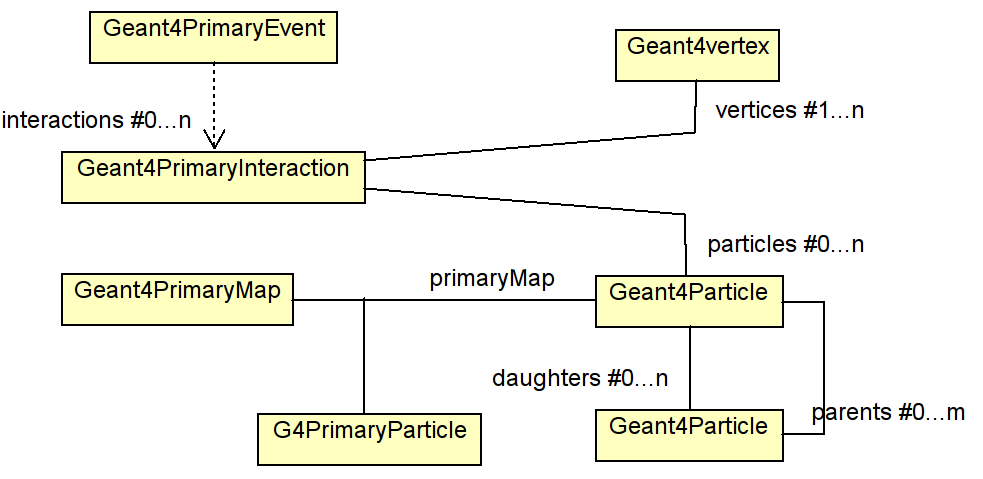
\includegraphics[width=120mm] {DDG4_event_data_model}
    \caption{The DDG4 event data model.}
    \label{fig:ddg4-event-data-model}
  \end{center}
\end{figure}

\noindent
{\bf{Please note}}, that this data model  is by no means to be made persistent 
and used for physics user analysis. This model is optimized to support
the simulation process and the necessary user actions to handle MC truth,
to easily and relatively fast look up and modify parent-daughter 
relationships etc. This choice is based on the assumption, that the 
additional overhead to convert particles at the input/output 
stage is small compared to the actual resource consumption of Geant4
to simulate the proper detector response.
On the other hand this choice has numerous advantages:
\begin{itemize}\itemcompact
\item Accepting the fact to convert input records allows to adapt 
  DDG4 in a simple and flexible manner to any input format. Currently 
  supported is the input from raw {\tts{LCIO}} files, {\tts{StdHep}} 
  records using {\tts{LCIO}} and {\tts{ASCII}} files using the 
  {\tts{HEPEvt}} format.
\item Similarly as for the input stage, also the output format 
  can be freely chosen by the clients.
\item No assumptions was made concerning the structure to store 
  information from energy deposits. Any information extract produced
  by the sensitive actions can be adapted provided at the output
  stage the proper conversion mechanism is present. The sensitive 
  detectors provided by DDG4 are {\bf{optional only and by no means mandatory}}.
  User defined classes may be provided at any time. Appropriate tools
  to extract MC truth information is provided at the output stage.
\item The modular approach of the action sequences described 
  in~\ref{sec:ddg4-user-manual-implementation-geant4action-sequences}
  allows to easily extend the generation sequence to handle multiple 
  simultaneous interactions, event overlay or spillover response 
  very easily~\footnote{The handling of spillover is only possible 
  if during the digitization step the correct signal shape corresponding
  to the shift of signal creation is taken into account.}
\end{itemize}

\noindent
In section~\ref{sec:ddg4-implementation-input-handling} the generic mechanism
of input data handling is described. \\
In section~\ref{sec:ddg4-implementation-particle-handling} the MC truth 
handling is discussed. \\
In section~\ref{sec:ddg4-implementation-output-handling} we describe the 
output mechanism.
\newpage

%=============================================================================
\subsection{Input Data Handling}
\label{sec:ddg4-implementation-input-handling}
%=============================================================================
\begin{figure}[t]
  \begin{center}
    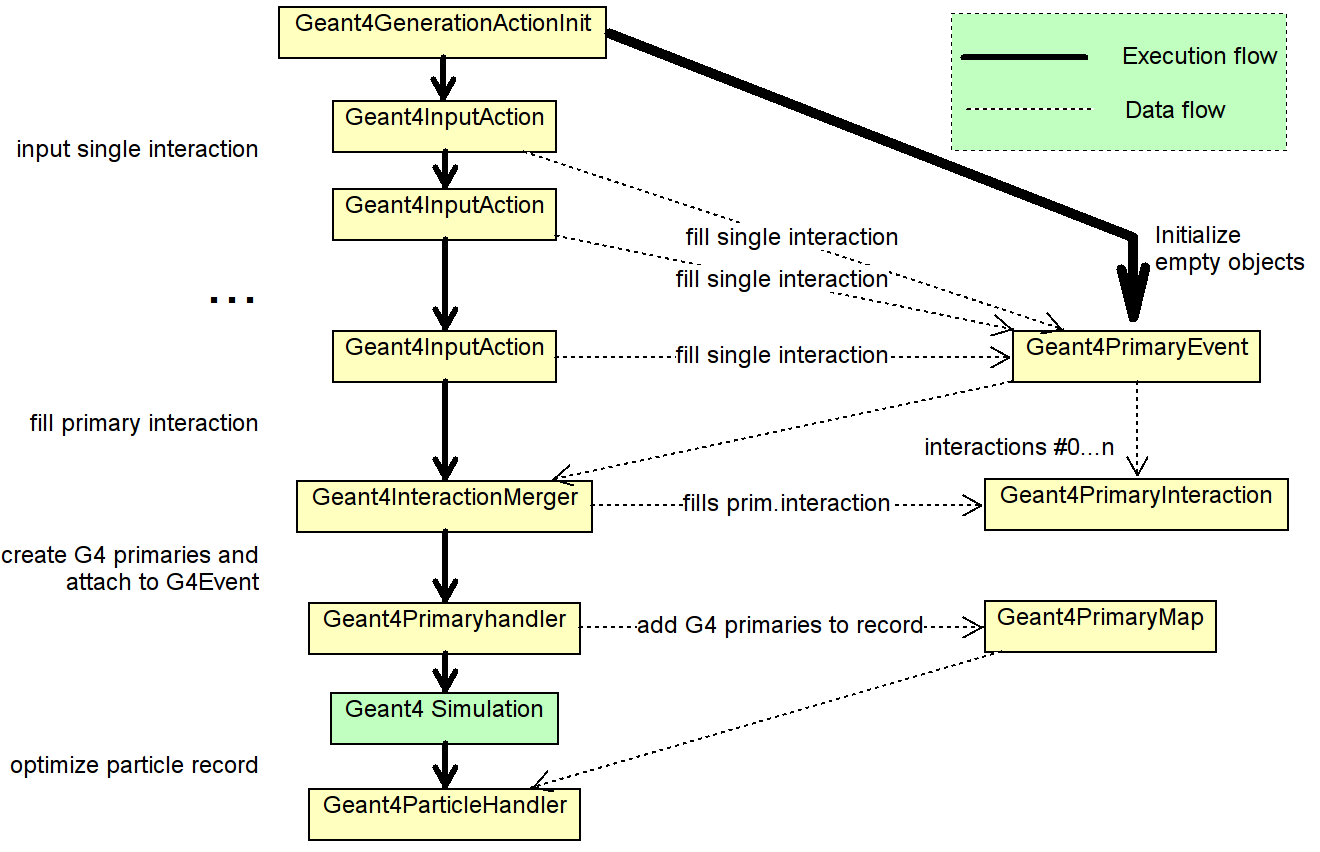
\includegraphics[width=160mm] {DDG4_input_stage}
    \caption{The generic handling of input sources to DDG4.}
    \label{fig:ddg4-input-stage}
  \end{center}
\end{figure}

\noindent
Input handling has several stages and uses several modules:
\begin{itemize}\itemcompact
\item First the data structures \tts{Geant4PrimaryEvent}, 
    \tts{Geant4PrimaryInteraction} and \tts{Geant4\-Primary}\-\tts{Map} are initialized 
    by the action \tts{Geant4GenerationActionInit} 
    and attached to the {\tts{Geant4Event}} structure.
\item The initialization is then followed by any number of input modules.
  Typically each input module add one interaction. Each interaction has a 
  unique identifier, which is propagated later to all particles. Hence all
  primary particles can later be unambiguously be correlated to one of the 
  initial interactions. 
  Each instance of a \tts{Geant4InputAction} creates and fills a separate instance
  of a \tts{Geant4PrimaryInteraction}.
  In section~\ref{sec:ddg4-implementation-geant4inputaction} the functionality and
  extensions are discussed in more detail.
\item All individual primary interactions are then merged to only single record
  using the \tts{Geant4}\-\tts{Interaction}\-\tts{Merger} component.
  This components fills the \tts{Geant4PrimaryInteraction} registered to the
  \tts{Geant4Event}, which serves as input record for the next component,
\item the \tts{Geant4PrimaryHandler}. The primary handler creates the proper 
  \tts{G4PrimaryParticle} and \tts{G4PrimaryVertex} objects passed to \tts{Geant4}.
  After this step all event related user interaction with Geant4 has completed,
  and the detector simulation may commence.
\end{itemize}
All modules used are subclasses of the {\tts{Geant4}\-\tts{Generator}\-\tts{Action}} and must be
added to the \tts{Geant4}\-\tts{Generator}\-\tts{Action}\-\tts{Sequence} as described 
in~\ref{sec:ddg4-user-manual-implementation-geant4action-sequences}.

\noindent
An object of type {\tts{Geant4PrimaryEvent}} exists exactly once for 
every event to be simulated. The empty {\tts{Geant4PrimaryEvent}} is created by the
{\tts{Geant4GenerationActionInit}} component. All higher level components may then 
access the {\tts{Geant4PrimaryEvent}} object and subsequently an individual interaction
from the {\tts{Geant4Context}} using the extension mechanism as shown in 
the following code:
\begin{code}
/// Event generation action callback
void SomeGenerationComponent::operator()(G4Event* event)  {
  /// Access the primary event object from the context
  Geant4PrimaryEvent* evt = context()->event().extension<Geant4PrimaryEvent>();
  /// Access the container of interactions
  const std::vector<Geant4PrimaryEvent::Interaction*>& inter = evt->interactions();
  /// Access one single interaction to be manipulated by this component
  Geant4PrimaryInteraction* evt->get(m_myInteraction_identifier);
  ....
\end{code}
{\bf{Please note:}} To keep components simple, each component should 
only act on one interaction the component has to uniquely identify.
The identification may be implemented by e.g. an access mask passed to the 
component as a property.

%=============================================================================
\subsection{Anatomy of the Input Action}
\label{sec:ddg4-implementation-geant4inputaction}
%=============================================================================
\noindent
One input action fills one primary interaction.
\tts{Geant4InputAction} instances may be followed by decorators, which 
allow to to smear primary vertex (\tts{Geant4InteractionVertexSmear}) or
to boost the primary vertex \tts{Geant4InteractionVertexBoost} and all 
related particles/vertices.


Please note, that a possible reduction of particles in
the output record may break this unambiguous relationship between 
"hits" and particles.
......

%=============================================================================
\subsection{Monte-Carlo Truth Handling}
\label{sec:ddg4-implementation-particle-handling}
%=============================================================================
As any other component in \DDG, the   was
designed using the plugin mechanism ie. the default implementation
which was inspired by the original implementation of the MC thruth
handler developed by the Linear Collider community may easily be
overloaded.

\noindent
The Monte-Carlo thruth handler takes care that 
\begin{itemize}
\item the proper MC particles are associated with the corresponding hits
      and tracks.
\item To compress the particle record. Geant4 creates a large amount 
      of temporary particles in particluar in dense areas of the 
      detector such as calorimeters. In calorimeters however, the 
      hits within a confined volume should be assigned to the incoming
      track. In addition a track is only supposed to be kept if it 
      satisfies certain criteria.
\end{itemize}
To achieve this functionality the Monte-Carlo thruth handler implemented
in the class \tts{Geant4ParticleHandler} firstly
\begin{itemize}
\item implements the interface \tts{Geant4MonteCarloTruth} which gets
      called whenever an interaction occurs in a sensitive volume
      which is modeled by an instance of a instance of 
      \tts{Geant4SensitiveAction}.
\item to properly manager the MC particle records the 			
	  \tts{Geant4ParticleHandler} either inherits or uses
	  the callbacks provided by the DDG4 interfaces to the
	  \begin{itemize}
		  \item \tts{Geant4GeneratorAction}
		  \item \tts{Geant4EventAction}
		  \item \tts{Geant4TrackingAction}
		  \item \tts{Geant4SteppingAction}.
	  \end{itemize}
	  While the response of one track is simulated, all relevant 
	  information is extracted in the callbacks and at the end of the
	  simulation of the track response a decision is taken whether to
	  store the information of the Geant4 track in the MC particle
	  record or not.
\item A Geant4 track is saved in the MC track record if
	  \begin{itemize}
	  	  \item the track did not intercat with the detector, but 
	  	  		is part of the Monte-Carlo record originating
	  	  		from the original generator consisting of quarks,
	  	  		leptons, gluons, gammas etc.
		  \item the track was declared to Geant4 as a Geant4 primary
		        track from the generator action. These are either 
		        long-living remnants of the underlying hard interaction
		        of particles decaying macroscopically inside the
		        experiment volume like e.g. B-mesons.
		  \item the track exits the world volume.
		  \item the track is mother particle to secondaries.
		  \item the track created a hit in a \it{"tracker"}-type
		        sensitive volume.
		  \item the track is above a certain energy threshold and
		  		has at least one associated hit either in a 
		  		\it{calorimter}-type volume of a \it{tracker}-type
		  		volume.
	  \end{itemize}
	  For all tracks purged from the MC particle record, any resulting
	  energy deposit is associated to the last parent particle 
	  stored in the MC particle record.
\item To fine-tune the Monte-Carlo truth handler in \DDG a 
	  use class with interface  \tts{Geant4UserParticleHandler} 
	  may be supplied, which allows to customize and fine tune
	  if a given MC particle is supposed to be kept in the final
	  record or not. This user class receives the identical callbacks
	  as the truth handler, but at the end of the simulation of each
	  track (the end-tracking-action) a call is issued by the truth
	  handler and allows to override the decision whether to keep
	  or dismiss storing a track.
\end{itemize}

\noindent
As mentioned above this implementation is only an example how
to realize such a Monte-Carlo truth logic. It is assumed that the
interface \tts{Geant4ParticleHandler} together with the easy-to-use
subscription mechanism to all callbacks provided by Geant4
allow to easily implement other Monte-Carlo truth mechanisms.

\vspace{0.3cm}
\noindent
The following table shows all properties accepted by the 
\DDG Monte-Carlo truth handler.

\vspace{0.3cm}
\noindent
\begin{tabular}{ l p{10cm} }
\hline
\bold{Class name}      & \tts{Geant4ParticleHandler}           \\
\bold{File name}       & \tts{DDG4/src/Geant4ParticleHandler.cpp} \\
\bold{Type}            & \tts{Geant4Action}                                  \\
\hline 
\bold{Component Properties:}   & defaults apply                              \\
\bold{PrintEndTracking} (bool) & \tts{Extra printout at the end of the } \\
                               & \tts{tracking action for debugging} \\
\bold{PrintStartTracking} (bool) & \tts{Extra printout at the start of the } \\
                               & \tts{tracking action for debugging} \\
\bold{KeepAllParticles} (bool) & \tts{Flag to override any NC particle removal} \\
\bold{SaveProcesses} (bool)    & \tts{Save all produces of the specified} \\
                               & \tts{Geant4 particle processes} \\
\bold{MinimalKineticEnergy} (bool)  & \tts{Minimal energy cut required to accept a MC particle} \\
\bold{MinDistToParentVertex} (bool) & \tts{Minimal distance to the parent's }\\
                               & \tts{start-vertex in order to become an independent particle} \\
                               & \tts{Used to e.g. suppress Delta-rays} \\
\end{tabular}

\newpage

%=============================================================================
\section{Output Data Handling}
\label{sec:ddg4-implementation-output-handling}
%=============================================================================

\noindent
The output of the data record of the accepted MC particle record
and the corresponding sets of hits in the various subdetectors is 
basic to further handing data originating from simulated particle
collisions. In \DDG the handling of output data is implemented as
a specialization of a \tts{Geant4EventAction} since the output
needs to written at the end of each simulated event.

\noindent
Currently there are three types of output formats implemented:
\begin{itemize}
\item Writing the MC particle record and the Geant4 hits
	  natively as ROOT objects to a ROOT file.
	  This is a very simple solution, writes the entire event
	  as a ROOT TTree object. The persistent data format of the 
	  objects is the same as the transition data format in memory
	  used during the simulation step.
\item Writing the particle record and the hit structures in LCIO 
      data format. For details of the LCIO data format
      please consult the LCIO manual.
\item Writing the particle record and the hit structures in 
      the EDMS data format developed by the CERN/SFT data format.
      For details of the LCIO data format please consult the LCIO
      manual.
\end{itemize}

Unless the native ROOT format is used for data output,
the data format of the transient representation 
of Monte-Carlo particles and the resulting tracker- and
calorimeter hits differes from the persistent representation 
and requires data conversion. The overheads of such conversions however
are typically neglidgeble with respect to the rather large resource
usage required for simulation.

\vspace{0.3cm}
\noindent
The component properties of the generic output class:

\vspace{0.3cm}
\noindent
\begin{tabular}{ l p{10cm} }
\hline
\bold{Class name}      & \tts{Geant4OutputAction}           \\
\bold{File name}       & \tts{DDG4/src/Geant4OutputAction.cpp} \\
\bold{Type}            & \tts{Geant4Action}                                  \\
\hline 
\bold{Component Properties:}   & defaults apply                              \\
\bold{Output} (string) & \tts{String representation of the output-file} \\
\bold{HandleErrorsAsFatal} (bool) & \tts{Convert any error of the concrete implementation}\\
                                  & \tts{into a fatal exception causing \DDG to stop processing.}\\
\end{tabular}

\vspace{0.3cm}
\noindent
The component properties of the ROOT output class:

\vspace{0.3cm}
\noindent
\begin{tabular}{ l p{10cm} }
\hline
\bold{Class name}      & \tts{Geant4Output2ROOT}           \\
\bold{File name}       & \tts{DDG4/src/Geant4Output2ROOT.cpp} \\
\bold{Type}            & \tts{Geant4Action}                                  \\
\hline 
\bold{Component Properties:}   & defaults apply                              \\
\bold{Section} (string)        & \tts{Name of the ROOT TTree to store the event data.}\\
                               & \tts{Default: EVENT} \\
\bold{HandleMCTruth} (bool)    & \tts{Handle the results of the Monte-Carlo thruth handler}\\
                               & \tts{when outputting data}\\
\bold{DisabledCollections}     & \tts{vector<string>}\\
                               & \tts{Geant4 filled collections, which should be excluded}\\
                               & \tts{from the output record.}\\
\bold{DisableParticles} (bool) & \tts{Inhibit the output of the particle record.}
                               
\end{tabular}


\newpage


%=============================================================================
\section{Multi-Threading in \DDG}
\label{sec:ddg4-multi-threading}
%=============================================================================
\subsection{Introductory Remarks}
\label{sec:ddg4-multi-threading-introduction}
%=============================================================================
\noindent
Multi-threading as supported by Geant4 is event driven. This means that 
the simulation of a given event is handled by one single thread.
Geant4 provides specific extensions to ease the users the use of its 
multi-threaded extensions~\cite{bib:Geant4-multi-threading}~\footnote{Please
note that the whole of Geant4 and your client code must be compiled with
the compile flag ${\tts{-DGEANT4_BUILD_MULTITHREADED=ON}}$}.
These extension divide in a formalized manner all actions to be performed
to setup a Geant4 multi-threaded program into

\begin{itemize}\itemcompact
\item {\bf{common}} actions to be performed and shared by all threads.
This includes the setup of the geometry and the physics list. The
other main area are
\item {\bf{thread-specific}} actions to be performed for each thread.
These are composed by the user actions called during the processing of
each run. These are the run-, event-, generation-, tracking-, 
stepping and stacking actions.
\end{itemize}

\noindent
To understand the interplay between \DDG and Geant4 let us quickly 
recapitulate the Geant4 mechanism how to configure multiple threads.
The setup of a multi-threaded application in Geant4 is centered around 
two additional classes, which both deal with single- and multi-threaded 
issues:

\begin{itemize}\itemcompact
\item {\tts{G4VUserActionInitialization}} class with 2 major callbacks:
	{\tts{Build()}} which is executed for each {\bf{worker thread}} and 
	{\tts{BuildForMaster()}} which is executed for master thread only.	
\item {\tts{G4VUserDetectorConstruction}} class with the callbacks
    {\tts{Construct()}}, where the shared geometry is constructed and
    {\tts{ConstructSDandField()}} where the sensitive detectors and the
    electro magnetic fields are provided.
\end{itemize}

\noindent
Both these Geant4 provided hooks are modeled in the standard \DDG 
way as action queues, which allow a modular and fine grained setup
as shown in Figure~\ref{fig:ddg4-user-initialization} and 
Figure~\ref{fig:ddg4-detector-initialization}.
\begin{figure}[t]
  \begin{center}
    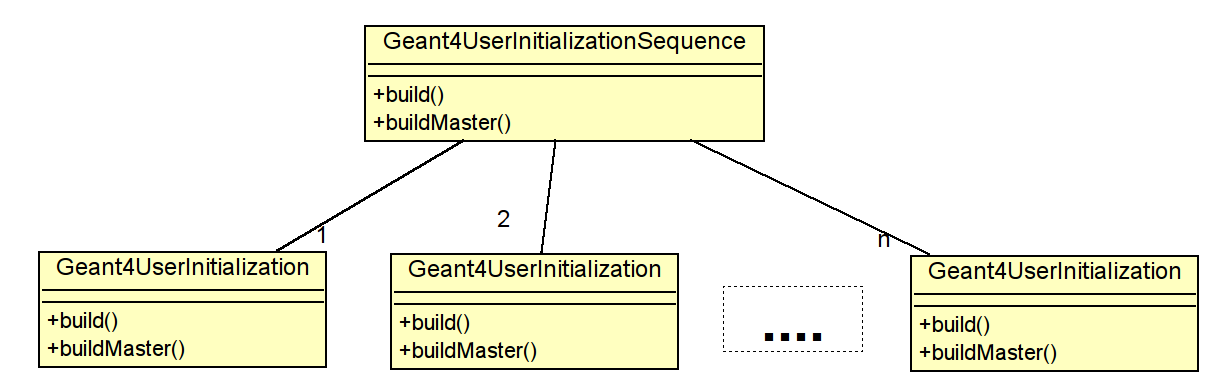
\includegraphics[width=140mm] {DDG4-User-Initialization}
    \caption{The Geant4 user initialization sequence to setup DDG4
             in multi-threaded mode. The callbacks {\tts{buildMaster()}} 
             is only called in multi-threaded mode.}
    \label{fig:ddg4-user-initialization}
  \end{center}
\end{figure}

\noindent
The \DDG framework ensures that all user callbacks are installed properly
to the Geant4 run manager, which calls them appropriately at the correct time.

\noindent
\DDG provides three callbacks for each sequence. Each callback receives
a temporary context argument, which may be used to shortcut access 
to basic useful quantities:
\begin{code}
    struct Geant4DetectorConstructionContext  {
      /// Reference to geometry object
      Geometry::LCDD&     lcdd;
      /// Reference to the world after construction
      G4VPhysicalVolume*  world;
      /// The cached geometry information
      Geant4GeometryInfo* geometry;
      /// G4 User detector initializer
      G4VUserDetectorConstruction* detector;
};
\end{code}

\begin{figure}[h]
  \begin{center}
    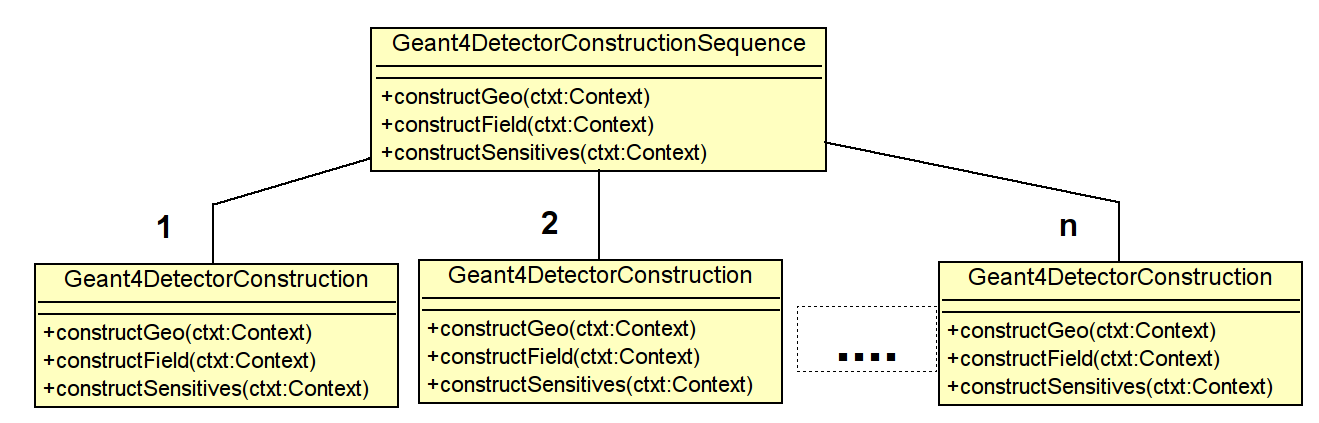
\includegraphics[width=140mm] {DDG4-Detector-Construction}
    \caption{The Geant4 detector initialization sequence to setup DDG4.
        If supplied, Geant4 calls the components both, in the single-threaded 
        and in the multi-threaded mode.}
    \label{fig:ddg4-detector-initialization}
  \end{center}
\end{figure}

The callbacks and the expected functionality are:
\begin{enumerate}
\item First the detector geometry is constructed. This happens in the callback
    {\tts{constructGeo(...)}}. If a standard \DDhep geometry 
    is present, this is translation of the geometry could be done by simply 
    calling the plugin {\tts{Geant4DetectorGeometryConstruction}}. 
    Alternatively a user defined plugin could perform this action.
\item Next the electromagnetic fields for the Geant4 particle tracking is
    constructed. A generic plugin {\tts{Geant4FieldTrackingConstruction}}
    may be attached. The corresponding setup parameters are listed in
    Section~\ref{sec:existing-ddg4-components}. 
    Alternatively a user defined plugin could perform this action.
\item Finally the Geant4 sensitive detectors are instantiated and attached 
    to the sensitive volumes. For generic setups the plugin
    {\tts{Geant4DetectorSensitivesConstruction}} may be attached.
    Alternatively a user defined plugin could perform this action.
\end{enumerate}

%=============================================================================
\subsection{Thread related contexts}
\label{sec:ddg4-thread-save context}
%=============================================================================
\noindent
\DDG provides thread related context, which may be accessed or modified
by user code. This context, the {\tts{Geant4Context}} and its sub-components,
as discussed in Section~\ref{sec:ddg4-implementation-higher-level-components}
are available as separate instances for each event and as such
also independently for each worker thread. Hence, no user level locking of the 
event context is necessary in any worker thread.

%=============================================================================
\subsection{Thread-Shared Components}
\label{sec:ddg4-multi-threaded-shared-actions}
%=============================================================================
\noindent
Some actions, though executed in the context of a single thread context 
may only execute as singletons. An example would be a {\tts{GeneratorAction}},
which read input events from file. Clearly the reading of data from
file must be protected and the reading of one event in a given thread
must finish, before the next thread may take over.
Another example are data analysis components, which e.g. fill a histogram.
Typically the filling mechanism of a histogram is not thread safe and hence must
be protected.

\noindent
To solve such issues all actions, which may involve such shared 
activities, a shared action is provided, which adopts a singleton
instance and executes the relevant callbacks in a protected manner.
The shared actions execute the user component in a thread safe envelope.

\noindent
Clearly no run- or event related state in such shared actions may be
carried by the component object across callbacks. The action objects
may not be aware of the event related context outside the callback.
Default implementations for such shared actions exist for
\begin{itemize}\itemcompact
\item the {\tts{Geant4RunAction}}, where the calls to 
        {\tts{Geant4RunAction::begin}} and {\tts{Geant4RunAction::end}}
        are {\bf{globally}} locked and the sequential execution of 
        the entire sequence is ensured;
\item the {\tts{Geant4EventAction}},
\item the {\tts{Geant4TrackingAction}},
\item the {\tts{Geant4SteppingAction}} and
\item the {\tts{Geant4StackingAction}}.
\end{itemize}
In the latter cases the framework ensures thread safety, but does 
not ensure the reentrant execution order of the entire sequence.

\noindent
{\bf{General Remark:}}
\noindent
Simple callbacks registered to the run-, event, etc.-actions cannot 
be protected. These callbacks may under no circumstances use any 
event related state information of the called object.

%=============================================================================
\subsection{Backwards- and Single-Thread-Compatibility}
\label{sec:ddg4-multi-threading-backwards}
%=============================================================================
\noindent
As in the single threaded mode of Geant4, also in the multi-threaded
mode all user actions are called by an instance of the {\tts{G4RunManager}}
or a sublass thereof, the {\tts{G4MTRunManager}}~\cite{bib:Geant4-multi-threading}.

\noindent
If the recommended actions in sub-section~\ref{sec:ddg4-multi-threading-introduction}
are used to configure the Geant4 application, then in a rather transparent
way both single-threaded and multi-threaded setups can coexist simply by 
changing the concrete instance of the {\tts{G4RunManager}}. There is one
single exception: The user initialization function
{\tts{G4VUserActionInitialization::BuildForMaster()}} is {\bf{only}} executed
in multi-threaded mode. For this reason, we deprecate the usage. Try
to find solutions, without master specific setup using e.g. shared actions.

%=============================================================================
\subsection{Support for Python Setup in Multi-Threading Mode}
\label{sec:ddg4-multi-threading-python}
%=============================================================================
\noindent
The setup of \DDG in multi-threaded mode requires separate callbacks for 
the global configuration (geometry, etc.) and the configuration of the worker 
threads. In python this setup is performed within {\rm{python callable}}
objects, which are either functions or member functions of objects.
These functions may have arguments. The python specific configuration actions
\begin{itemize}\itemcompact
\item The user initialization action 
    {\tts{Geant4PythonInitialization}} allows to configure python callbacks
    for the master and the worker thread setup using the calls:
    \begin{code}
      /// Set the Detector initialization command
      void setMasterSetup(PyObject* callable, PyObject* args);
      /// Set the field initialization command
      void setWorkerSetup(PyObject* callable, PyObject* args);              \end{code}
     to be used in python as a call sequence within the master thread:
    \begin{code}
     init_seq = kernel.userInitialization(True)
     init_action = UserInitialization(kernel,'Geant4PythonInitialization/PyG4Init')
     init_action.setWorkerSetup(worker_setup_call, < worker_args > )
     init_action.setMasterSetup(master_setup_call, < master_args > )
     init_seq.adopt(init_action)                                            \end{code}
    The callback argument list $< worker\_args >$ and $< master\_args >$
    are python tuples containing all arguments expected by the callable objects
    $worker\_setup\_call$ and $master\_setup\_call$ respecyively.
    The class {\tts{Geant4PythonInitialization}} is a subclass of
    {\tts{Geant4UserInitialization}} and will call the provided functions
    according to the protocol explained earlier in this section.
    If a callback is not set, the corresponding actiion is not executed.
\item The detector construction action 
    {\tts{Geant4PythonDetectorConstruction}} is the corresponding 
    python action to populate the detector construction sequencer.
    and supports three ccallbacks:
    \begin{code}
      /// Set the Detector initialization command
      void setConstructGeo(PyObject* callable, PyObject* args);
      /// Set the field initialization command
      void setConstructField(PyObject* callable, PyObject* args);
      /// Set the sensitive detector initialization command
      void setConstructSensitives(PyObject* callable, PyObject* args);    \end{code}
    to be used in python as call sequence within the master thread:
    \begin{code}
    init_seq = self.master().detectorConstruction(True)
    init_action = DetectorConstruction(self.master(),name_type)
    init_action.setConstructGeo(geometry_setup_call, < geometry_args > )
    init_action.setConstructField(field_setup_call, < field_args > )
    init_action.setConstructSensitives(sensitives_setup_call, < sensitives_args >)
    init_seq.adopt(init_action)                                           \end{code}
    If any of the three callback is not set, the corresponding actiion is not executed.
    Hereby are $geometry\_setup\_call$, $field\_setup\_call$ and $sensitives\_setup\_call$ 
    the callable objects to configure the geometry, the tracking field 
    and the sensitive detectors.
    $< geometry\_args >$, $< field\_args >$ and $< sensitives\_args >$ are 
    the corresponding callable arguments in the form of a python tuple object.   
\end{itemize}

\noindent
All python callbacks are supposed to return the integer '1' on success.
Any other return code is assumed to be failure.

%=============================================================================
\subsection{\DDG Multi-Threading Example}
\label{sec:ddg4-multi-threading-example}
%=============================================================================
\begin{code}
"""

   DD4hep simulation example setup DDG4
   in multi-threaded mode using the python configuration

   @author  M.Frank
   @version 1.0

"""
import os, time, DDG4

def setupWorker(geant4):
  kernel = geant4.kernel()
  print '#PYTHON: +++ Creating Geant4 worker thread ....'
  print "#PYTHON:  Configure Run actions"
  run1 = DDG4.RunAction(kernel,'Geant4TestRunAction/RunInit')
    ...
  print "#PYTHON:  Configure Event actions"
  prt = DDG4.EventAction(kernel,'Geant4ParticlePrint/ParticlePrint')
  kernel.eventAction().adopt(prt)
    ...
  print "\n#PYTHON:  Configure I/O\n"
  evt_root = geant4.setupROOTOutput('RootOutput','CLICSiD_'+time.strftime('%Y-%m-%d_%H-%M'))
    ...
  gen = DDG4.GeneratorAction(kernel,"Geant4GeneratorActionInit/GenerationInit")
  kernel.generatorAction().adopt(gen)
  print "#PYTHON:  First particle generator: pi+"
  gen = DDG4.GeneratorAction(kernel,"Geant4IsotropeGenerator/IsotropPi+");
    ...
  print "#PYTHON:  Merge all existing interaction records"
  gen = DDG4.GeneratorAction(kernel,"Geant4InteractionMerger/InteractionMerger")
  kernel.generatorAction().adopt(gen)
  print "#PYTHON:  Finally generate Geant4 primaries"
  gen = DDG4.GeneratorAction(kernel,"Geant4PrimaryHandler/PrimaryHandler")
  kernel.generatorAction().adopt(gen)
  print "#PYTHON:  ....and handle the simulation particles."
  part = DDG4.GeneratorAction(kernel,"Geant4ParticleHandler/ParticleHandler")
  kernel.generatorAction().adopt(part)

  user = DDG4.Action(kernel,"Geant4TCUserParticleHandler/UserParticleHandler")
    ...
  part.adopt(user)
  print '#PYTHON: +++ Geant4 worker thread configured successfully....'
  return 1
  
def setupMaster(geant4):
  kernel = geant4.master()
  print '#PYTHON: +++ Setting up master thread for ',kernel.NumberOfThreads,' workers.'
  return 1

def setupSensitives(geant4):
  print "#PYTHON:  Setting up all sensitive detectors"
  geant4.printDetectors()
  print "#PYTHON:  First the tracking detectors"
  seq,act = geant4.setupTracker('SiVertexBarrel')
    ...
  print "#PYTHON:  Now setup the calorimeters"
  seq,act = geant4.setupCalorimeter('EcalBarrel')
    ...
  return 1

def run():
  kernel = DDG4.Kernel()
  lcdd = kernel.lcdd()
  install_dir = os.environ['DD4hepINSTALL']
  DDG4.Core.setPrintFormat("%-32s %6s %s")
  kernel.loadGeometry("file:"+install_dir+"/DDDetectors/compact/SiD.xml")
  DDG4.importConstants(lcdd)

  kernel.NumberOfThreads = 3
  geant4 = DDG4.Geant4(kernel,tracker='Geant4TrackerCombineAction')
  print "#  Configure UI"
  geant4.setupCshUI()

  print "#  Geant4 user initialization action"
  geant4.addUserInitialization(worker=setupWorker, worker_args=(geant4,),
                               master=setupMaster,master_args=(geant4,))
  print "#  Configure G4 geometry setup"
  seq,act = geant4.addDetectorConstruction("Geant4DetectorGeometryConstruction/ConstructGeo")

  print "# Configure G4 sensitive detectors: python setup callback"
  seq,act = geant4.addDetectorConstruction("Geant4PythonDetectorConstruction/SetupSD",
                                           sensitives=setupSensitives,sensitives_args=(geant4,))
  print "# Configure G4 sensitive detectors: atach'em to the sensitive volumes"
  seq,act = geant4.addDetectorConstruction("Geant4DetectorSensitivesConstruction/ConstructSD")

  print "#  Configure G4 magnetic field tracking"
  seq,field = geant4.addDetectorConstruction("Geant4FieldTrackingConstruction/MagFieldTrackingSetup")
  field.stepper            = "HelixGeant4Runge"
  field.equation           = "Mag_UsualEqRhs"
  field.eps_min            = 5e-05 * mm
  ...
  print "#  Setup random generator"
  rndm = DDG4.Action(kernel,'Geant4Random/Random')
  rndm.Seed = 987654321
  rndm.initialize()
  print "#  Now build the physics list:"
  phys = geant4.setupPhysics('QGSP_BERT')
  geant4.run()

if __name__ == "__main__":
  run()
\end{code}

\newpage

%=============================================================================
\section{Existing DDG4 components}
\label{sec:existing-ddg4-components}
%=============================================================================
\noindent
In the introduction the longterm goal was expressed, that with DDG4 users
should be able to pick components from a growing palette and connect the
selected components using the setup mechanisms described in 
Section~\ref{sec:ddg4-implementation-setup}.

\noindent
Such a palette based approach obviously depends on the availability of
documentation for existing components describing the properties
of each component and the interaction of each component within the \DDG
framework.

\noindent
All components defer from the basic type \tts{Geant4Action}. This means 
\bold{all} components have the \bold{default} properties described in the
table below:

\vspace{0.5cm}
\noindent
\begin{tabular}{ l l p{9cm} }
\hline
Component Properties: &  & \tts{default} \\
\hline
\bold{OuputLevel}     & [int]  & Output level of the component to customize printouts             \\
\bold{Name}           & [string]  & Component name [read-only] \\
\bold{Control}        & [boolean] & Steering of the Geant4 Messenger creation \\
\hline
\end{tabular}


\vspace{5cm}

\begin{center}
{\large{\bf{
\begin{tabular} {| p{15cm} |}
\hline\space  \\

\noindent
{\underline{Important notice for developers:}} \\

\noindent
Since the documentation of developed components is VERY important,
please never forget to supply the corresponding documentation.\\
\\
\noindent
At least supply the minimal documentation ash shown below
in the appended examples for the "Simple" detector response and I/O
components.
\\ \space\hline 
\end{tabular}
}}}
\end{center}
\clearpage

%=============================================================================
\subsection{Generic Action Modules}
%=============================================================================

%=============================================================================
\subsubsection{Geant4UIManager}
%=============================================================================
\noindent
The {\tt{Geant4UIManager}} handles interactivity aspects between Geant4,
its command handlers (i.e. terminal) and the various components the actions
interact.

\noindent
The {\tt{Geant4UIManager}} is a component attached to the {\tt{Geant4Kernel}}
object. All properties of all {\tt{Geant4Action}} instances may be exported to 
\tts{Geant4} messengers and {\em{may}} hence be accessible directly from 
the \tts{Geant4} prompt. To export properties from any action, call the 
{\tt{enableUI()}} method of the action.
\noindent
The callback signature is: \tts{void operator()(G4Event* event)}.

\vspace{0.5cm}
\noindent
\begin{tabular}{ l p{10cm} }
\hline
\bold{Class name}      & \tts{Geant4UIManager}                           \\
\bold{File name}       & \tts{DDG4/src/Geant4UIManager.cpp}              \\
\bold{Type}            & \tts{Geant4Action}                              \\
\hline
\bold{Component Properties:}   & defaults apply                          \\
\hline
\bold{SessionType} (string)  & Session type (csh, tcsh, etc.             \\
\bold{SetupUI} (string)   & Name of the UI macro file                    \\
\bold{SetupVIS} (string)  & Name of the visualization macro file         \\
\bold{HaveVIS} (bool)     & Flag to instantiate Vis manager 
                            (def:false, unless VisSetup set)             \\
\bold{HaveUI} (bool)      & Flag to instantiate UI (default=true)        \\
\end{tabular}

%=============================================================================
\subsubsection{Geant4Random}
%=============================================================================
\noindent
Mini interface to the random generator of the application.
Necessary, that on every object creates its own instance, but accesses
the main instance available through the \tts{Geant4Context}.

\noindent
This is mandatory to ensure reproducibility of the event generation
process. Particular objects may use a dependent generator from
an experiment framework like \tts{GAUDI}.

\noindent
internally the engine factory mechanism of \tts{CLHEP} is used. Please refer
there within for valid engine names and the random seeding mechanism,
which may vary between different engines.

\noindent
Any number of independent random objects may be created and used 
in parallel. This however, is not advised to ensure reproducibility.

\noindent
The first instance of the random action is automatically set
to be the \tts{Geant4} instance. If another instance should be used by 
\tts{Geant4}, use \tts{setMainInstance(Geant4Random* ptr)} class method to 
override this behavior.
Provision, steered by options, is taken to ensure the \tts{gRandom}
of \tts{ROOT} uses the same random number engine.

\vspace{0.5cm}
\noindent
\begin{tabular}{ l p{10cm} }
\hline
\bold{Class name}                & \tts{Geant4Random}                             \\
\bold{File name}                 & \tts{DDG4/src/Geant4Random.cpp}                \\
\bold{Type}                      & \tts{Geant4Random}                             \\
\hline
\bold{Component Properties:}     & defaults apply                                 \\
\hline
\bold{File}   (string)           & File name if initialized from file.            \\
                                 & If set, engine name and seeds are ignored      \\
\bold{Engine} (string)           & Engine type name.                              \\
                                 & All engines defined in the
                                   \tts{CLHEP::EngineFactory} class are available.
                                   If no type is supplied the engine from the 
                                   HepRandom generator instance is taken.         \\
\bold{Seed}   (long)             & Initial random seed.                           \\
                                 & Default:    123456789.                         \\
                                 & If not ZERO terminated, termination is added.  \\
\bold{Replace\_gRandom} (bool)   & Flag to replace the \tts{ROOT} \tts{gRandom}
                                   instance with this random number engine.
                                   This ensures \tts{ROOT} and \tts{Geant4} 
                                   use the same random number engine, hence 
                                   the same random sequence.
                                                                                  \\
\end{tabular}

\noindent
%=============================================================================
\subsection{Geant4UserInitialization Implementations}
%=============================================================================
\noindent
%=============================================================================
\subsubsection{Geant4PythonInitialization}
%=============================================================================
\noindent
Please see Section~\ref{sec:ddg4-multi-threading-python} 
for an illustration of the usage.
The configuration by construction must be performed using setter-functions
rather than properties.

\vspace{0.5cm}
\noindent
\begin{tabular}{ l p{10cm} }
\hline
\bold{Class name}      & \tts{Geant4PythonInitialization}                    \\
\bold{File name}       & \tts{DDG4/src/python/Geant4PythonInitialization.cpp} \\
\bold{Type}            & \tts{Geant4Action}                                  \\
\hline 
\bold{Component Properties:}   & defaults apply                              \\
\end{tabular}

%=============================================================================
\subsubsection{Geant4PythonDetectorConstruction}
%=============================================================================
\noindent
Please see Section~\ref{sec:ddg4-multi-threading-python} 
for an illustration of the usage.
The configuration by construction must be performed using setter-functions
rather than properties.

\vspace{0.5cm}
\noindent
\begin{tabular}{ l p{10cm} }
\hline
\bold{Class name}      & \tts{Geant4PythonDetectorConstruction}              \\
\bold{File name}       & \tts{DDG4/src/python/Geant4PythonDetectorConstruction.cpp}  \\
\bold{Type}            & \tts{Geant4Action}                                  \\
\hline 
\bold{Component Properties:}   & defaults apply                              \\
\end{tabular}

%=============================================================================
\subsection{Predefined Geant4 Physics List Objects}
%=============================================================================
\noindent
The physics list may be defined entirely data driven using the factory mechanism
using a variety of predefined objects. Though users are free to define private 
physics lists, typically the predefined physics lists from \tts{Geant4} are used. 

\noindent
The inventory changes over time, new lists appear and obsolete lists are purged,
hence we will not list them explicitly here.
For the inventory of available physics lists, please refer to the implementation files:

\noindent
\begin{itemize}\itemcompact
\item Inventory of predefined physics lists, which may be inherited:\\
\detdesc{html/_geant4_physics_lists_8cpp_source.html}
{DDG4/plugins/Geant4PhysiscsLists.cpp}
\item Inventory of predefined physics constructors, which may be instantiated:\\
\detdesc{html/_geant4_physics_constructors_8cpp_source.html}
{DDG4/plugins/Geant4PhysicsConstructors.cpp}
\item Inventory of predefined process constructors, which may be instantiated:\\
\detdesc{html/_geant4_processes_8cpp_source.html}
{DDG4/plugins/Geant4Processes.cpp}
\item Inventory of predefined particle constructors, which may be instantiated:\\
\detdesc{html/_geant4_particles_8cpp_source.html}
{DDG4/plugins/Geant4Particles.cpp}
\end{itemize}
\newpage

%=============================================================================
\subsection{Geant4 Generation Action Modules}
%=============================================================================
\noindent
Here we discuss modules, which are intrinsically part of DDG4 and may be
attached to the {\tt{Geant4GeneratorActionSequence}}.

%=============================================================================
\subsubsection{Base class: Geant4GeneratorAction}
%=============================================================================
\noindent
The \tts{Geant4GeneratorAction} is called for every event.
During the callback all particles are created which form the 
microscopic kinematic action of the particle collision.
This input may either origin directly from an event generator program
or come from file.

\noindent
The callback signature is: void operator()(G4Event* event)
\noindent
See also:
\detdesc{html/class_d_d4hep_1_1_simulation_1_1_geant4_generator_action.html}
{\tts{Geant4EventAction}} in the doxygen documentation.

\vspace{0.5cm}
\noindent
\begin{tabular}{ l p{10cm} }
\hline
\bold{Class name}      & \tts{Geant4GeneratorAction}                     \\
\bold{File name}       & \tts{DDG4/src/Geant4GeneratorAction.cpp}        \\
\bold{Type}            & \tts{Geant4Action, Geant4GeneratorAction}       \\
\hline
\bold{Component Properties:}   & defaults apply                          \\
\hline
\end{tabular}

%=============================================================================
\subsubsection{Geant4GeneratorActionSequence}
%=============================================================================
\noindent
The sequence dispatches the callbacks at the beginning 
of an event to all registered \tts{Geant4GeneratorAction} members and all 
registered callbacks.

\noindent
See also:
\noindent
The {\tt{Geant4GeneratorActionSequence}} is directly steered by the single
instance of the {\tt{G4VUserPrimaryGeneratorAction}}, the Geant4 provided user hook,
which is private.\\
See also:
\detdesc{html/struct_d_d4hep_1_1_simulation_1_1_geant4_user_generator_action.html}
{\tts{Geant4UserGeneratorAction}} and
\detdesc{html/class_d_d4hep_1_1_simulation_1_1_geant4_generator_action_sequence.html}
{\tts{Geant4GeneratorActionSequence}} in the doxygen documentation.

\vspace{0.5cm}
\noindent
\begin{tabular}{ l p{10cm} }
\hline
\bold{Class name}      & \tts{Geant4Geant4GeneratorActionSequence}       \\
\bold{File name}       & \tts{DDG4/src/Geant4GeneratorAction.cpp}        \\
\bold{Type}            & \tts{Geant4Action}                              \\
\hline
\bold{Component Properties:}   & defaults apply                          \\
\hline
\end{tabular}

%=============================================================================
\subsubsection{Geant4GeneratorActionInit}
%=============================================================================
\noindent
Initialize the Geant4Event objects to host generator and MC truth related information
Geant4 actions to collect the MC particle information.
This action should register all event extension required for the further 
processing. We want to avoid that every client has to check if a given 
object is present or not and than later install the required data structures.

\noindent
These by default are extensions of type:
\begin{itemize}\itemcompact
\item \tts{Geant4PrimaryEvent} with multiple interaction sections, one for each interaction
    This is the MAIN and ONLY information to feed Geant4
\item \tts{Geant4PrimaryInteraction} containing the track/vertex information to create 
    the primary particles for Geant4. This record is build from the \tts{Geant4PrimaryEvent}
    information.
\item \tts{Geant4PrimaryMap} a map of the \tts{Geant4Particles} converted to 
    \tts{G4PrimaryParticles} to ease particle handling later.
\item \tts{Geant4ParticleMap} the map of particles created during the event simulation.
    This map has directly the correct particle offsets, so that the merging of
    \tts{Geant4PrimaryInteraction} particles and the simulation particles is easy....
\end{itemize}

\vspace{0.5cm}
\noindent
\begin{tabular}{ l p{10cm} }
\hline
\bold{Class name}      & \tts{Geant4Geant4GeneratorActionInit}           \\
\bold{File name}       & \tts{DDG4/src/Geant4GeneratorActionInit.cpp}    \\
\bold{Type}            & \tts{Geant4GeneratorAction}                     \\
\hline
\bold{Component Properties:}   & defaults apply                            \\
\bold{Angle} (double)          & \tts{Lorentz-Angle of boost}                          \\
\bold{Mask} (int.bitmask)      & \tts{Interaction identifier} \\
\hline
\end{tabular}

%=============================================================================
\subsubsection{Geant4InteractionVertexBoost}
%=============================================================================
\noindent
Boost the primary vertex and all particles outgoing the primary interaction in X-direction.

\noindent
The interaction to be processed by the component is uniquely identified
by the {\bf{Mask}} property. Two primary interaction may not have the same
mask.

\noindent
{\bold{Note [special use case]:}}\\
If all contributing interactions of the one event \bold{registered 
in the primary event at the time the action is called} should be handled by 
one single component instance, set the {\bf{Mask}} property to {\bold{-1}}.

\vspace{0.5cm}
\noindent
\begin{tabular}{ l p{10cm} }
\hline
\bold{Class name}        & \tts{Geant4InteractionVertexBoost}              \\
\bold{File name}         & \tts{DDG4/src/Geant4InteractionVertexBoost.cpp} \\
\bold{Type}              & \tts{Geant4GeneratorAction}                     \\
\hline
\bold{Component Properties:}   & defaults apply                            \\
\bold{Angle} (double)          & \tts{Lorentz-Angle of boost}              \\
\bold{Mask} (int.bitmask)      & \tts{Interaction identifier}              \\
\hline
\end{tabular}

%=============================================================================
\subsubsection{Geant4InteractionVertexSmear}
%=============================================================================
\noindent
Smear the primary vertex and all particles outgoing the primary interaction.

\noindent
The interaction to be processed by the component is uniquely identified
by the {\bf{Mask}} property. Two primary interaction may not have the same
mask.

\noindent
{\bold{Note [special use case]:}}\\
If all contributing interactions of the one event \bold{registered 
in the primary event at the time the action is called} should be handled by 
one single component instance, set the {\bf{Mask}} property to {\bold{-1}}.

\vspace{0.5cm}
\noindent
\begin{tabular}{ l p{10cm} }
\hline
\bold{Class name}        & \tts{Geant4InteractionVertexSmear}              \\
\bold{File name}         & \tts{DDG4/src/Geant4InteractionVertexSmear.cpp} \\
\hline
\bold{Component Properties:}   & defaults apply                            \\
\bold{Offset}  (PxPyPzEVector) & \tts{Smearing offset}                     \\
\bold{Sigma}   (PxPyPzEVector) & \tts{Sigma (Errors) on offset}            \\
\bold{Mask}    (int.bitmask)   & \tts{Interaction identifier} \\
\hline
\end{tabular}

%=============================================================================
\subsubsection{Geant4InteractionMerger}
%=============================================================================
\noindent
Merge all interactions created by each {\tt{Geant4InputAction}} into one single
record. The input records are taken from the item {\tt{Geant4PrimaryEvent}}
and are merged into the {\tt{Geant4PrimaryInteraction}} object attached to the
{\tt{Geant4Event}} event context.

\vspace{0.5cm}
\noindent
\begin{tabular}{ l p{10cm} }
\hline
\bold{Class name}        & \tts{Geant4InteractionMerger}                   \\
\bold{File name}         & \tts{DDG4/src/Geant4InteractionMerger.cpp}      \\
\bold{Type}              & \tts{Geant4GeneratorAction}                     \\
\hline
\bold{Component Properties:}   & defaults apply                            \\
\hline
\end{tabular}

%=============================================================================
\subsubsection{Geant4PrimaryHandler}
%=============================================================================
\noindent
Convert the primary interaction (object {\tt{Geant4PrimaryInteraction}} object 
attached to the {\tt{Geant4Event}} event context) and pass the result
to Geant4 for simulation.

\vspace{0.5cm}
\noindent
\begin{tabular}{ l p{10cm} }
\hline
\bold{Class name}        & \tts{Geant4PrimaryHandler}                      \\
\bold{File name}         & \tts{DDG4/src/Geant4PrimaryHandler.cpp}         \\
\bold{Type}              & \tts{Geant4GeneratorAction}                     \\
\hline
\bold{Component Properties:}   & defaults apply                            \\
\hline
\end{tabular}

%=============================================================================
\subsubsection{Geant4ParticleGun}
%=============================================================================
\noindent
Implementation of a particle gun using Geant4Particles.

\noindent
The {\tt{Geant4ParticleGun}} is a tool to shoot a number of
particles with identical properties into a given region of the
detector to be simulated.

\noindent
The particle gun is a input source like any other and participates 
in the general input stage merging process like any other input 
e.g. from file. Hence, there may be several particle guns present
each generating it's own primary vertex. Use the mask property to
ensure each gun generates it's own, well identified primary vertex.

\noindent
There is one 'user lazyness' support though:
If there is only one particle gun in use, the property 'Standalone', 
which by default is set to true invokes the interaction merging and the
Geant4 primary generation directly.

\noindent
The interaction to be created by the component is uniquely identified
by the {\bf{Mask}} property. Two primary interaction may not have the same
mask.

\vspace{0.5cm}
\noindent
\begin{tabular}{ l p{10cm} }
\hline
\bold{Class name}         & \tts{Geant4PrimaryHandler}                      \\
\bold{File name}          & \tts{DDG4/src/Geant4PrimaryHandler.cpp}         \\
\bold{Type}               & \tts{Geant4GeneratorAction}                     \\
\hline
Component Properties:     & default                                         \\
\bold{particle} (string)  & Particle type to be shot                        \\
\bold{energy} (double)    & Particle energy in $MeV$                        \\
\bold{position} (XYZVector)  & Pole position of the generated particles in $mm$\\
\bold{direction} (XYZVector) & Momentum direction of the generated particles\\
\bold{isotrop} (bool)        & Isotropic particle directions in space.      \\
\bold{Mask} (int.bitmask)    & Interaction identifier                       \\
\bold{Standalone} (bool)     & Setup for standalone execution               \\ 
                             & including interaction merging etc.           \\
\hline
\end{tabular}

%=============================================================================
\subsubsection{Geant4ParticleHandler}
%=============================================================================
\noindent
Extract the relevant particle information during the simulation step.

\noindent
This procedure works as follows:
\begin{itemize}\itemcompact
\item At the beginning of the event generation the object registers itself as 
    Monte-Carlo truth handler to the event context.
\item At the begin of each track action a particle candidate is created and filled
    with all properties known at this time.
\item At each stepping action a flag is set if the step produced secondaries.
\item Sensitive detectors call the MC truth handler if a hit was created.
    This fact is remembered.
\item At the end of the tracking action a first decision is taken if the candidate is to be 
    kept for the final record.
\item At the end of the event action finally all particles are reduced to the 
    final record. This logic can be overridden by a user handler to be attached.
\end{itemize}
\noindent
Any of these actions may be intercepted by a {\tt{Geant4UserParticleHandler}}
attached to the particle handler.
See class {\tt{Geant4UserParticleHandler}} for details.

\vspace{0.5cm}
\noindent
\begin{tabular}{ l p{9cm} }
\hline
\bold{Class name}      & \tts{Geant4ParticleHandler}                     \\
\bold{File name}       & \tts{DDG4/src/Geant4ParticleHandler.cpp}        \\
\bold{Type}            & \tts{Geant4GeneratorAction}                     \\
\hline
\bold{Component Properties:}   & defaults apply                            \\
\bold{KeepAllParticles} (bool)    & Flag to keep entire particle record without any reduction.
                            This may result in a huge output record.      \\
\bold{SaveProcesses} (vector(string)) & Array of Geant4 process names, 
                            which products and parent should NOT be reduced.\\
\bold{MinimalKineticEnergy} (double) & Minimal energy below which particles should be
                            ignored unless other criteria 
                            (Process, created hits, etc) apply.\\
\hline
\end{tabular}
\newpage

%=============================================================================
\subsection{Geant4 Event Action Modules}
%=============================================================================
\noindent

%=============================================================================
\subsubsection{Base class: Geant4EventAction}
%=============================================================================
\noindent
The EventAction is called for every event.

\noindent
This class is the base class for all user actions, which have
to hook into the begin- and end-of-event actions.
Typical use cases are the collection/computation of event
related properties.

\noindent
Examples of this functionality may include for example:
\begin{itemize}\itemcompact
\item Reset variables summing event related information in the
  begin-event callback.
\item Monitoring activities such as filling histograms
  from hits collected during the end-event action.
\end{itemize}
See also:
\detdesc{html/class_d_d4hep_1_1_simulation_1_1_geant4_event_action.html}
{\tts{Geant4EventAction}} in the doxygen documentation.

\vspace{0.5cm}
\noindent
\begin{tabular}{ l p{10cm} }
\hline
\bold{Class name}      & \tts{Geant4EventAction}                     \\
\bold{File name}       & \tts{DDG4/src/Geant4EventAction.cpp}        \\
\bold{Type}            & \tts{Geant4EventAction}                     \\
\hline
\bold{Component Properties:}   & defaults apply                        \\
\hline
\end{tabular}

%=============================================================================
\subsubsection{Geant4EventActionSequence}
%=============================================================================
\noindent

\noindent
The {\tt{Geant4EventActionSequence}} is directly steered by the single
instance of the {\tt{G4UserEventAction}}, the Geant4 provided user hook,
which is private.\\
See also:
\detdesc{html/struct_d_d4hep_1_1_simulation_1_1_geant4_user_event_action.html}
{\tts{Geant4UserEventAction}} in the doxygen documentation.

\vspace{0.5cm}
\noindent
\begin{tabular}{ l p{10cm} }
\hline
\bold{Class name}      & \tts{Geant4EventAction}                     \\
\bold{File name}       & \tts{DDG4/src/Geant4EventAction.cpp}        \\
\bold{Type}            & \tts{Geant4EventAction}                     \\
\hline
\bold{Component Properties:}   & defaults apply                      \\
\hline
\end{tabular}

%=============================================================================
\subsubsection{Geant4ParticlePrint}
%=============================================================================
\noindent
Geant4Action to print MC particle information.

\vspace{0.5cm}
\noindent
\begin{tabular}{ l p{10cm} }
\hline
\bold{Class name}      & \tts{Geant4ParticlePrint}                     \\
\bold{File name}       & \tts{DDG4/src/Geant4ParticlePrint.cpp}        \\
\bold{Type}            & \tts{Geant4EventAction}                       \\
\hline
\bold{Component Properties:}   & defaults apply                        \\
\bold{OutputType} (bool)       & Flag to steer output type.            \\
                                & 1: Print table of particles.          \\
                                & 2: Print table of particles.          \\
                                & 3: Print table and tree of particles. \\
\bold{PrintHits} & Print associated hits to every particle (big output!)\\
\hline
\end{tabular}
\newpage


%=============================================================================
\subsection{Sensitive Detectors}
%=============================================================================
\noindent

%=============================================================================
\subsubsection{Geant4TrackerAction}
%=============================================================================
\noindent
Simple sensitive detector for tracking detectors. These trackers create one
single hit collection. The created hits may be written out with the output
modules described in Section~\ref{sec:ddg4-components-IO-ROOT-simple} 
and~\ref{sec:ddg4-components-IO-LCIO-simple}. \\
The basic specifications are:

\vspace{0.5cm}
\noindent
\begin{tabular}{ l p{10cm} }
\hline
Basics: & \\
\hline
\bold{Class name}      & \tts{Geant4SensitiveAction<Geant4Tracker>}  \\
\bold{File name}       & \tts{DDG4/plugins/Geant4SDActions.cpp}      \\
\bold{Hit collection}  & \tts{Name of the readout object}            \\
\bold{Hit class}       & \tts{Geant4Tracker::Hit}                    \\
\bold{File name}       & \tts{DDG4/include/Geant4Data.h}             \\
\hline
\bold{Component Properties:}   & defaults apply                       \\
\hline
\end{tabular}

%=============================================================================
\subsubsection{Geant4CalorimeterAction}
%=============================================================================
\noindent
Simple sensitive detector for calorimeters. The sensitive detector creates one
single hit collection. The created hits may be written out with the output
modules described in Section~\ref{sec:ddg4-components-IO-ROOT-simple} 
and~\ref{sec:ddg4-components-IO-LCIO-simple}. \\
The basic specifications are:

\vspace{0.5cm}
\noindent
\begin{tabular}{ l p{10cm} }
\hline
Basics: & \\
\hline
\bold{Class name}      & \tts{Geant4SensitiveAction<Geant4Calorimeter>}  \\
\bold{File name}       & \tts{DDG4/plugins/Geant4SDActions.cpp}      \\
\bold{Hit collection}  & \tts{Name of the readout object}            \\
\bold{Hit class}       & \tts{Geant4Calorimeter::Hit}                \\
\bold{File name}       & \tts{DDG4/include/Geant4Data.h}             \\
\hline
\bold{Component Properties:}   & defaults apply                       \\
\hline
\end{tabular}

\newpage

%=============================================================================
\subsection{I/O Components}
%=============================================================================
\noindent

%=============================================================================
\subsubsection{ROOT Output "Simple"}
\label{sec:ddg4-components-IO-ROOT-simple}
%=============================================================================
\noindent

%=============================================================================
\subsubsection{LCIO Output "Simple"}
\label{sec:ddg4-components-IO-LCIO-simple}
%=============================================================================
\noindent



%=============================================================================
\newpage
\begin{thebibliography}{9}
\bibitem{bib:DD4hep}  DD4Hep web page, http://aidasoft.web.cern.ch/DD4hep.

\bibitem{bib:LHCb} 		LHCb Collaboration, 
                "LHCb, the Large Hadron Collider beauty experiment, reoptimised detector 
				design and performance", CERN/LHCC 2003-030

\bibitem{bib:LHCb-geometry} S. Ponce et al., 
                "Detector Description Framework in LHCb", 
                International Conference on Computing in High Energy and Nuclear Physics  (CHEP 2003), 
                La Jolla, CA, 2003, proceedings. 

\bibitem{bib:ILD}  The ILD Concept Group, 
                   "The International Large Detector: Letter of Intent",\\
                   ISBN 978-3-935702-42-3, 2009.

\bibitem{bib:SiD}  H. Aihara, P. Burrows, M. Oreglia (Editors),
                   "SiD Letter of Intent",
                   arXiv:0911.0006, 2009.

\bibitem{bib:ROOT-tgeo} R.Brun, A.Gheata, M.Gheata, "The ROOT geometry package",\\
                    Nuclear Instruments and Methods {\bf{A}} 502 (2003) 676-680.

\bibitem{bib:ROOT} R.Brun et al., 
                   "Root - An object oriented data analysis framework",\\
                    Nuclear Instruments and Methods {\bf{A}} 389 (1997) 81-86.

\bibitem{bib:geant4}  S. Agostinelli et al., 
                   "Geant4 - A Simulation Toolkit", \\
                    Nuclear Instruments and Methods {\bf{A}} 506 (2003) 250-303.

\bibitem{bib:LCDD} T.Johnson et al., 
                   "LCGO - geometry description for ILC detectors", 
                   International Conference on Computing in High Energy and Nuclear Physics  (CHEP 2007), 
                   Victoria, BC, Canada, 2012, Proceedings.

\bibitem{bib:lcsim} N.Graf et al., 
                   "lcsim: An integrated detector simulation, 
                   reconstruction and analysis environment", 
                   International Conference on Computing in High Energy and Nuclear Physics (CHEP 2012),
                   New York, 2012, Proceedings.

\bibitem{bib:GDML} R. Chytracek et al.,
                   "Geometry Description Markup Language for Physics Simulation and Analysis
                   Applications",
                   IEEE Trans. Nucl. Sci., Vol. 53, Issue: 5, Part 2, 2892-2896,
                   http://gdml.web.cern.ch.

\bibitem{bib:DDSegmentations} C.Grefe et al.,
                   "The DDSegmentation package", 
                   Non existing documentation to be written.
\bibitem{bib:Geant4-multi-threading} Geant4 Multi threading Guides. 
	Please see for details:\\
	https://twiki.cern.ch/twiki/bin/view/Geant4/Geant4MTAdvandedTopicsForApplicationDevelopers,\\
	https://twiki.cern.ch/twiki/bin/view/Geant4/QuickMigrationGuideForGeant4V10,\\
	http://geant4.slac.stanford.edu/tutorial/MC2015G4WS/Multithreading.pdf

\end{thebibliography}
%=============================================================================
\end{document}
